%%%% ijcai21.tex

\typeout{IJCAI--21 Instructions for Authors}

% These are the instructions for authors for IJCAI-21.

\documentclass{article}
\pdfpagewidth=8.5in
\pdfpageheight=11in
% The file ijcai21.sty is NOT the same than previous years'
\usepackage{ijcai21}

% Use the postscript times font!
\usepackage{times}
\usepackage{soul}
\usepackage{url}
\usepackage{microtype}
\usepackage[hidelinks]{hyperref}
\usepackage[utf8]{inputenc}
\usepackage[small]{caption}
\usepackage{graphicx}
\usepackage{booktabs}
\usepackage{algorithm}
\usepackage{algorithmic}
\usepackage{courier}
\usepackage{color}
\usepackage{amsmath,amsfonts,amssymb,amsthm,amsopn}
\usepackage{epsfig}
\usepackage{booktabs}
\usepackage{array}
\usepackage{multicol}
\usepackage{threeparttable}
\usepackage{epstopdf}
\usepackage{listings}
\usepackage{multirow}
\usepackage{subfigure}
\usepackage{ragged2e}
\usepackage{xassoccnt}

\renewcommand{\algorithmicrequire}{ \textbf{Input:}}
\renewcommand{\algorithmicensure}{ \textbf{Output:}} 
\newcommand{\KZ}[1]{\textcolor{blue}{Kenny: #1}}

\urlstyle{same}

% the following package is optional:
%\usepackage{latexsym}

% See https://www.overleaf.com/learn/latex/theorems_and_proofs
% for a nice explanation of how to define new theorems, but keep
% in mind that the amsthm package is already included in this
% template and that you must *not* alter the styling.
\newtheorem{example}{Example}
\newtheorem{theorem}{Theorem}

% Following comment is from ijcai97-submit.tex:
% The preparation of these files was supported by Schlumberger Palo Alto
% Research, AT\&T Bell Laboratories, and Morgan Kaufmann Publishers.
% Shirley Jowell, of Morgan Kaufmann Publishers, and Peter F.
% Patel-Schneider, of AT\&T Bell Laboratories collaborated on their
% preparation.

% These instructions can be modified and used in other conferences as long
% as credit to the authors and supporting agencies is retained, this notice
% is not changed, and further modification or reuse is not restricted.
% Neither Shirley Jowell nor Peter F. Patel-Schneider can be listed as
% contacts for providing assistance without their prior permission.

% To use for other conferences, change references to files and the
% conference appropriate and use other authors, contacts, publishers, and
% organizations.
% Also change the deadline and address for returning papers and the length and
% page charge instructions.
% Put where the files are available in the appropriate places.

%PDF Info Is REQUIRED.
\pdfinfo{
/TemplateVersion (IJCAI.2021.0)
}

\title{Automatic Paraphrasing via Sentence Reconstruction and
Back-translation}

% Single author syntax
% \author{
%     Zhi-Hua Zhou
%     \affiliations
%     Nanjing University
%     \emails
%     pcchair@ijcai-21.org
% }

% Multiple author syntax (remove the single-author syntax above and the \iffalse ... \fi here)
% Check the ijcai21-multiauthor.tex file for detailed instructions
\iffalse
\author{
First Author$^1$
\and
Second Author$^2$\and
Third Author$^{2,3}$\And
Fourth Author$^4$
\affiliations
$^1$First Affiliation\\
$^2$Second Affiliation\\
$^3$Third Affiliation\\
$^4$Fourth Affiliation
\emails
\{first, second\}@example.com,
third@other.example.com,
fourth@example.com
}
\fi

\begin{document}

\maketitle

\begin{abstract}
Paraphrase generation plays key roles in NLP tasks such as question answering, machine translation, and information retrieval. In this paper, we propose a novel framework for paraphrase generation. It simultaneously decodes the output sentence using a pretrained wordset-to-sequence model and a back-translation model. We evaluate this framework on Quora, WikiAnswers, MSCOCO and Twitter, and show its advantage over previous state-of-the-art unsupervised methods and distantly-supervised methods by significant margins on all datasets. For Quora and WikiAnswers, our framework even performs better than some strongly supervised methods with domain adaptation. Further, we show that the generated paraphrases can be used to augment the training data for machine translation to achieve substantial improvements.
\end{abstract}

%\IEEEraisesectionheading{
% %\IEEEraisesectionheading{
% %\IEEEraisesectionheading{
% \input{intro}
\section{Introduction}\label{sec:intro}
 %}
% \section{Introduction}\label{sec:intro}

% \begin{enumerate}
% \item Motivation: application scenarios (with 1-2 running examples);
% \item Characteristics of the data sources and their challenges;
% \item Briefly introduce previous approaches to extract information 
% from images including setting the document zone, and their limitations.
% \item General flow of our approach (may give a diagram here)
% \end{enumerate}
% scenary

Due to ever evolving hardware and software, many medical images
such as electro-cardio graphs (ECGs), X-ray or ultrasound images  
are directly printed and stored in hard copy formats. 
% \KZ{Insert 4 example images here.}
%Examples are shown in \figref{fig:medicalImages}. 
% These images often contain a mix of graphics and text, which
% include parameter settings of the hardware, test measurements or simple
% diagnosis. 
These images often contain a mix of graphics and text, which 
include technical settings of the hardware used, test measurements or simple diagnoses.
Recently, there has been a growing demand for digitizing such 
medical information from paper media sources, especially legacy ones, or patients who want to keep track of these documents by themselves digitally. 
Apart from scanning the graphics into a digital format, extracting 
the semi-structured textual information is also an important part of
building electronic medical records for patients. 

%\begin{figure}[!htb]
%\centering
%\subfloat[ECG]{
%\label{fig:medicalimage:ecg}
%\epsfig{file=figure/17_ori.eps, width=0.4\columnwidth}
%}
%% \hfill
%\subfloat[MRI]{
%	\label{fig:medicalimage:mrt}
%	\epsfig{file=figure/MRI.eps, width=0.4\columnwidth}
%}
%\\
%\subfloat[X-RAY]{
%\label{fig:medicalimage:xray}
%\epsfig{file=figure/X-RAY.eps, width=0.4\columnwidth}
%}
%%\hfill
%\subfloat[EEG]{
%\label{fig:medicalimage:eeg}
%\epsfig{file=figure/EEG.eps, width=0.4\columnwidth}
%}
%\caption{Examples of Medical Images}
%\label{fig:medicalImages}
%\end{figure}

Optical character recognition (OCR)  \cite{mori1992historical,smith2007overview} is 
a traditional technique used to turn images of printed text into machine encoded
text. It is well researched and performs well on plain text 
documents such as novels and reports, for a variety of languages. 
%For example, Tesseract, which is one of 
%the most popular open source multilingual recognizers, logs an error 
%rate of 3.72\% for English words and 3.77\% for simplified 
%Chinese characters\cite{smith2009adapting}. 
%Google Books \cite{googlebooks} and Gutenberg \cite{gutenberg} are
%projects which have scanned a large number of paper books into text for free and open
%access. These projects made exclusive use of OCR for this conversion and 
%achieved high accuracy \cite{vincent2007google} \cite{lebert2008project}. 
% 99\% for Gutenberg project \cite{lebert2008project}. 
% \KZ{Give the accuracy of google and gutenberg if available.}


\begin{figure}[th]
\centering
\epsfig{file=figure/17_b.eps, width=0.8\columnwidth}
\caption{An ECG image with text area (red circle) of interest.}
\label{fig:ecgexample2}
\end{figure}

For a semi-structured medical image, such as 
\figref{fig:ecgexample2}, we would like to extract the attribute-value 
pairs (e.g., {\em Vent. rate = 63 bpm}) and possibly other values such as
date ({\em 18-Nov-2010}) and time ({\em 9:13:02}) since those values endow us with lots of information about the patient. 
Existing OCR software cannot extract such structured information in a straightforward 
fashion, 
but instead it produces rather convoluted results from the whole image, 
similar to those in \figref{fig:ocrre}, which was produced by Tesseract, 
a popular multi-lingual recognizers. 
% \KZ{Maybe include the x-y coordinate info in the output as well?}  

\begin{figure}[th]
\centering
\scriptsize
\begin{verbatim}
<p class="ocr_par" title="box 263 33 444 119">
   <span class="ocr_l" title="box 264 33 336 45">
       <span class="ocrx_w" title="box 264 33 299 45">Vcnt.</span> 
       <span class="ocrx_w" title="box 308 34 336 45">rule</span> 
   </span>
   <span class='ocr_l'>
       <span class="ocrx_w" title="box 264 51 283 64">PR</span> 
       <span class="ocrx_w" title="box 291 51 346 64">Interval</span> 
       <span class="ocrx_w" title="box 389 52 411 64">140</span> 
       <span class="ocrx_w" title="box 420 55 439 64">ms</span> 
   </span>
   ...
   </span>
</p>
<p class="ocr_p" dir="ltr">
   <span class="ocr_l">
       <span class="ocrx_w" title="box 396 33 411 45">53</span> 
       <span class="ocrx_w" title="box 420 33 449 48">bpm</span> 
   </span>
</p>
\end{verbatim}
\caption{Snippet OCR results in XML, input to our framework.}
\label{fig:ocrre}
\end{figure}


%\input{xmlre1}

%However, OCR alone does not work well on semi-structured text and hence
%can't be directly used for information extraction from the aforementioned
%medical images. \KZ{Give the reason here, perhaps because OCR models are
%largely Markov based? So semi-structured data breaks the flow of text.}
%When a medical image is input to an ordinary OCR software, the spatial 
%information of the text components is often lost or mixed with noises
%and errors.
%%The reason is OCR converts the whole images into text data, in which 
%%useful information often mix with noises and errors. 
%In this paper, we would like to extract the attribute-value pairs
%and possibly other values from \figref{fig:ecgexample1} 
%and \figref{fig:ecgexample2}. 
%% or medical ultrasonography report. 
%Such images contain lots of non-textual information or noises.

% example & ref
%\begin{figure}[ht]
%\centering
%\epsfig{file=figure/46.eps, width=0.8\columnwidth}
%\caption{ECG Images From Printer1}
%\label{fig:ecgexample1}
%\end{figure}

% \begin{figure}[ht]
% \centering
% \subfloat[Printer1]{
% \label{fig:ecgexample:a}
% \epsfig{file=figure/46.eps, width=0.48\columnwidth}
% }
% \hfill
% \subfloat[Printer2]{
% \label{fig:ecgexample:b}
% \epsfig{file=figure/17.eps, width=0.48\columnwidth}
% }
% \caption{ECG images from two different printers}
% \label{fig:ecgexample}
% \end{figure}

Also, errors in the OCR text \cite{darwish2007error,taghva1996evaluation} will greatly affect the effectiveness 
of other related tasks. Much work has been done to improve the performance of the OCR\cite{kolak2003generative,cesarini1998informys}. However, there are still a number of significant challenges involved in extracting the information from medical images or OCR results in XML form. 

% First, medical images differ from pure text document in that them have 
% layout information. 
First, medical images differ from pure text documents in that 
they contain layout information.
Although most current OCR engines attempt to reproduce the physical 
layout of the text units, 
%(along with X-Y coordinates) and store them 
%in a special format such as XML 
% (\KZ{Better in the previous example})
such spatial
information is approximate and sometimes inaccurate, which is why neighboring
text blocks in \figref{fig:ecgexample2}, such as ``Vent. Rate'' and
``63 bpm'' were not automatically combined into the same XML block, but were 
rather far apart (shown in two different ``classes'') in \figref{fig:ocrre} made by OCR softwares. 
%Even for images produced by the same ECG printer, 
%the XML results can still be very different as 
The spatial layout is sensitive to many factors, such as accidental spots 
on the prints, color and contrast, or the angle of the camera. 
%In this case, solutions for other application domains, for example, the web, 
%are not well suited for information extraction from printed documents \cite{bartoli2014semisupervised}. With such inaccurate
%layout information produced by OCR,
%it is not easy to write a simple wrapper program to extract useful
%data from images, even if the images come from the same printer. 

%Writing a wrapper for each
%individual image would be tedious and counter-productive. Therefore,
%a mechanism that makes use of the spatial locality of the 
%text units in the image and 
%accommodates slight variations in the spatial layout would make the extraction
%more accurate and fault-tolerant.

%For example, \figref{fig:ocrre} is the simplified OCR results for the ECGs in 
%\figref{fig:ecgexample1} and \figref{fig:ecgexample2}. The results are in the XML format and have attritube named {\em class} 
%for layout information. Although these two images share similar format. 
%OCR engine generates different results in that it splits elements that 
%should be in the same line into two lines in the second example. 
%XML is sensitive to the layout results so it's hard to tolerate 
%all the layout results. 
%
% example check the term
% layout of ocr results can be restore, so why OCR engine don't restore the results 
% using the similar methods as we do?
% or the way we handle the layout problem is quite simple

% Delete for TIP
% Second, exiting OCR engines make heavy use of Markov properties such as n-grams
% since they primarily target the transformation of large body of text 
% \cite{kolak2003generative}. 
% % \KZ{Needs some refs here.}
% Unfortunately, the semi-structured texts in medical images are often 
% short and not even written in complete sentences, thus breaking Markov assumption. To make
% matters worse, medical images contain scientific language, which may be
% very different from the training corpora of these OCR engines.
% This explains why we see errors like ``Vcnt'' and ``rule'' 
% in \figref{fig:ocrre}. 
% %can't guarantee a perfect performance, which means 
% %there are errors and noises in the OCR results.
% %Many of them due to the fact that the data are no longer long, continous
% %sentences, thus breaking the Markov assumption made by many OCR algorithms. 
% %In \figref{fig:ocrresub:b}, ``Vent." is misrecognized as ``Vcnt.". 
% Without sufficient contextual information, OCR may also misrecognize a 
% digit as an alphabetic character, or as another similar digit. 
% Furthermore, the mix of text with images and formatting
% lines often confuses the OCR engine, which is more biased toward full
% text images.
% Exact pattern matching, as used in
% traditional information extraction, doesn't work with such noisy OCR output
% as it doesn't tolerate noises or errors in text. 
% %It's hard to autocorrect these errors 
% %because image quality is the most important affecting factor. 
% %The text we are processing can be full of no meaning words or 
% %strange numbers. 
% A fuzzy matching strategy is more desirable in this case. 
% % example, what are the traditional IEs

Second, there are many types of medical images, resulting from a variety of
medical tests. Different equipments for the same test can produce vastly 
different images. Writing individual extraction wrappers 
for the OCR outputs of all these formats is tedious and inefficient, 
and difficult for non-programmers.
%not to mention that there are significant programming barriers for 
%writing these wrappers, especially for the medical professionals who are the
%end users of these extraction results. 
%A more user-friendly approach enabling users to specify such extraction requirements would be preferred. 
%There are various kinds of medical images, such as electrocardiograph report, 
%medical ultrasonography report, etc. 
%However the basic measures for each type of medical test (e.g., ECG), 
%are very similar from machine to machine. Only the layouts are 
%different. 
% example medical images

Finally, most off-the-shelf OCR programs are pre-trained with specific 
recognition models, which may not be suitable for the extraction of 
%medical images.
%Furthermore, changes in imaging equipment technology over time may produce 
%different formats, layout, or terminology, rendering existing OCR models 
%obsolete. 
Re-training the models requires a large amount of labeled data, which may
not be available. 
%Incremental training as more labeled data arrives
%is currently not supported by any OCR product.    

%There have been some limited attempts to address some of the above challenges. 
%One solution is a plugin of an OCR program that allows the user to specify 
%target zones of interest in the image to be extracted. The zones specified for
%one image can be applied to images with slight variations by adjusting against
%a fixed reference point that is supposed to exist in all these images.
%% \KZ{I think the problem is not so much with the zones, because we also
%% have zones, but rather with the reference point.}
%% \JY{}
%% example products
%% http://www.square-9.com/automated-data-extraction-optical-character-recognition
%The problem with this solution is its high reliance on the OCR zones  
%established by the user. The performance of the results is affected by the 
%accuracy of the zones. If the zones are too big, the results will be full of 
%noise. If the zones are too small, results will miss something. 
%
%Another solution involves using the page layout analysis technique. The page layout 
%analysis technique is used to determine where the text 
%resides on a page \cite{o1993document}, 
%% \KZ{This page layout analysis approach is not clearly described. I don't understand after reading this paragraph.}
%% By using page layout analysis technique, the hierarchy of physical components 
%% can be generated and to match with the hierarchy of logical components, which 
%% is predefined. 
%this includes identifying and categorizing the 
%regions of interest in the scanned image of a text document. 
%Typically, the first step is to segment text zones from 
%non-textual zones and arrange them in their original order. 
%Then in order to analyze the logical roles of the text zones 
%(titles, captions, footnotes, etc.), logical layout analysis 
%is used for labeling the semantics of the text zones.
%Generally, page layout analysis is used for documents. The problem with applying 
%such a technique on medical images is that it creates so much noises 
%that performance is ultimately affected. 
%For medical imaging reports like ECG, useful information is often 
%found in the small components of the image, while most of the images are 
%read as noises. 
% check paper and more description, weakness, ref

%In this paper, 
%we propose a spatial data description language, which borrows its syntax from
%PADS \cite{fisher+:pads}, an ad hoc data processing language, 
%for describing semi-structured data in medical images. 
%% ref
%We call this language OCR description language, or ODL. 
%ODL is designed for extracting and parsing semi-structured text data 
%from images. We believe that  information extraction from those data in ODL form may be much easier than extracting information from rough data or data in XML form, which means that our preprocessing part proves to be necessary.
%%An example ODL description for the image in 
%%\figref{fig:ecgexample2} is shown in 
%%\figref{fig:description}. \KZ{Make this description two column, and give
%%some brief explanation of this description here.} 
%%The parsing result of this description is shown
%%in \figref{fig:parsing result}. \KZ{Give some explanation of the results,
%%otherwise don't show the result here. E.g., you need to explain what F, E, etc.
%%mean. You want to say that even though rate has been recognized as rule,
%%the bpm value was still extracted (but still wrong!).}
%% \KZ{I removed the preprocessing part, cos it's not important. Talk about it in
%% discussion sec.}
%%The our approach starts by preprocessing the images for text results.
%To use this framework, the user first describes the components in the image
%that he or she is interested in extracting. This includes constant strings
%and variables of different data types.   
%ODL allows the user to specify the approximate spatial layout and constraints on
%the data, e.g., integers within 
%a certain range, real numbers with certain decimal points, etc. 
%%This information is then as the key component in our fuzzy matching strategy. 
%The system then automatically generates a parser for these medical images.
%This parser uses the output XML from OCR with spatial information as an input, 
%and outputs a data structure with values extracted for each variables
%in the description, unless there is an unrecoverable error during the parsing process.
%In addition, approximate layout information and constraints are used in parsing process 
%to tolerate noises and small format variations in the input images. 
%%Specifically, this method could be called fuzzy matching, meaning that more candidates could be saved after the parsing process.  It's obvious that we may have a higher probability to obtain the accurate result if more candidates are kept so that fuzzy match should be used properly in our system.
%%An autogenerated parser based on the ODL description can release us from 
%%repetitive work. In this way, we turn the task of writing complex parsers 
%%into describing information on images.
%
%
%When users process many images of the same format, the system 
%automatically discovers parsing errors given the current model and 
%prompts the user to manually correct some of the frequent and prominent
%errors, which effectively serves as an online labeling function. 
%These incrementally labeled data are then used to update the parsing model. 


%It should be emphasized that the incremental learning model is very important in our whole system. Incremental learning is a machine learning paradigm where the learning process takes place whenever we have new examples or data added to our baisc data set, leading to a most striking difference between incremental learning and traditional machine learning: it does not assume the availability of a sufficient training set before the learning process. What incremental learning in our system is really impressive: it does not require a relatively good and stable training set at first time. In fact, it could improve the parsing result with even relatively rough training sets at first by absorbing new data or corrective information as time passes in dynamic systems. Besides, the process would be very effective when there are some new images coming in since training process would not learn from scratch, which might waste time and computation resource.

%At last, we propose an incrementally human correction framwork which can 
%make the best use of human correction to handle the misrecognition problem. 
% Base on our experiments on about 500 real life ECG images, 
% our approach achieves p1 and p2 after p3 times human correction. 
% experimental results

% \begin{figure}[h]
% \begin{lstlisting}
% Oenum str_month_t{
% 	"Jan", "Feb", "Mar", "Apr",
% 	"May", "Jun", "Jul", "Aug",
% 	"Sept", "Oct", "Nov", "Dec"
% };

% Ounion month_t{
% 	Oint(1,12)	num;
% 	str_month_t	str;
% };

% Ostruct time_t{
% 	Oint(1,31)	day;
% 	"-";
% 	month_t	month;
% 	"-";
% 	Oint	year;
% };

% Ostruct triple_t{
% 	"Vent.";
% 	hskip(\s)	skip1;
% 	"rate";
% 	Oint x;
% 	"bpm";
% 	vskip(\n)	skip2;
% };

% Oscource Ostruct entry_t{
% 	time_t(<-,-,-,0.3l>) t;
% 	triple_t(<0.1w,-,0.5w,->) d;
% };
% \end{lstlisting}
% \caption{Description}\label{fig:description}
% \end{figure}


In order to solve above problems, We design a system which makes three main contributions:
\begin{enumerate}
\item Based on some previous work on data description language \cite{lamport1986document,taft1999post,fisher+:pads},we design a new declarative spatial data description language called \textit{OCR description language}, or ODL,
which allows users to specify spatial and data constraints in medical 
images(\secref{sec:syntax});
\item We propose a noise-tolerant parser which takes OCR results
the ODL description as input and outputs a data structure with values 
extracted for each variables in the description (\secref{sec:semantics});
\item We propose an incremental manual correction 
framework\cite{von2008recaptcha,zhu2012learnpads++}, which 
takes advantage of user corrections  and improves the productivity
significantly (\secref{sec:correction}).
%To be more specific, the framework improves the traditional machine learning methods by using a incremental learning process to avoid starting from scratch when we are trying to apply human corrections in the system. That means the framework would be more effective than most corrective systems.
\end{enumerate}


\section{Introduction}\label{sec:intro}
 %}
% \section{Introduction}\label{sec:intro}

% \begin{enumerate}
% \item Motivation: application scenarios (with 1-2 running examples);
% \item Characteristics of the data sources and their challenges;
% \item Briefly introduce previous approaches to extract information 
% from images including setting the document zone, and their limitations.
% \item General flow of our approach (may give a diagram here)
% \end{enumerate}
% scenary

Due to ever evolving hardware and software, many medical images
such as electro-cardio graphs (ECGs), X-ray or ultrasound images  
are directly printed and stored in hard copy formats. 
% \KZ{Insert 4 example images here.}
%Examples are shown in \figref{fig:medicalImages}. 
% These images often contain a mix of graphics and text, which
% include parameter settings of the hardware, test measurements or simple
% diagnosis. 
These images often contain a mix of graphics and text, which 
include technical settings of the hardware used, test measurements or simple diagnoses.
Recently, there has been a growing demand for digitizing such 
medical information from paper media sources, especially legacy ones, or patients who want to keep track of these documents by themselves digitally. 
Apart from scanning the graphics into a digital format, extracting 
the semi-structured textual information is also an important part of
building electronic medical records for patients. 

%\begin{figure}[!htb]
%\centering
%\subfloat[ECG]{
%\label{fig:medicalimage:ecg}
%\epsfig{file=figure/17_ori.eps, width=0.4\columnwidth}
%}
%% \hfill
%\subfloat[MRI]{
%	\label{fig:medicalimage:mrt}
%	\epsfig{file=figure/MRI.eps, width=0.4\columnwidth}
%}
%\\
%\subfloat[X-RAY]{
%\label{fig:medicalimage:xray}
%\epsfig{file=figure/X-RAY.eps, width=0.4\columnwidth}
%}
%%\hfill
%\subfloat[EEG]{
%\label{fig:medicalimage:eeg}
%\epsfig{file=figure/EEG.eps, width=0.4\columnwidth}
%}
%\caption{Examples of Medical Images}
%\label{fig:medicalImages}
%\end{figure}

Optical character recognition (OCR)  \cite{mori1992historical,smith2007overview} is 
a traditional technique used to turn images of printed text into machine encoded
text. It is well researched and performs well on plain text 
documents such as novels and reports, for a variety of languages. 
%For example, Tesseract, which is one of 
%the most popular open source multilingual recognizers, logs an error 
%rate of 3.72\% for English words and 3.77\% for simplified 
%Chinese characters\cite{smith2009adapting}. 
%Google Books \cite{googlebooks} and Gutenberg \cite{gutenberg} are
%projects which have scanned a large number of paper books into text for free and open
%access. These projects made exclusive use of OCR for this conversion and 
%achieved high accuracy \cite{vincent2007google} \cite{lebert2008project}. 
% 99\% for Gutenberg project \cite{lebert2008project}. 
% \KZ{Give the accuracy of google and gutenberg if available.}


\begin{figure}[th]
\centering
\epsfig{file=figure/17_b.eps, width=0.8\columnwidth}
\caption{An ECG image with text area (red circle) of interest.}
\label{fig:ecgexample2}
\end{figure}

For a semi-structured medical image, such as 
\figref{fig:ecgexample2}, we would like to extract the attribute-value 
pairs (e.g., {\em Vent. rate = 63 bpm}) and possibly other values such as
date ({\em 18-Nov-2010}) and time ({\em 9:13:02}) since those values endow us with lots of information about the patient. 
Existing OCR software cannot extract such structured information in a straightforward 
fashion, 
but instead it produces rather convoluted results from the whole image, 
similar to those in \figref{fig:ocrre}, which was produced by Tesseract, 
a popular multi-lingual recognizers. 
% \KZ{Maybe include the x-y coordinate info in the output as well?}  

\begin{figure}[th]
\centering
\scriptsize
\begin{verbatim}
<p class="ocr_par" title="box 263 33 444 119">
   <span class="ocr_l" title="box 264 33 336 45">
       <span class="ocrx_w" title="box 264 33 299 45">Vcnt.</span> 
       <span class="ocrx_w" title="box 308 34 336 45">rule</span> 
   </span>
   <span class='ocr_l'>
       <span class="ocrx_w" title="box 264 51 283 64">PR</span> 
       <span class="ocrx_w" title="box 291 51 346 64">Interval</span> 
       <span class="ocrx_w" title="box 389 52 411 64">140</span> 
       <span class="ocrx_w" title="box 420 55 439 64">ms</span> 
   </span>
   ...
   </span>
</p>
<p class="ocr_p" dir="ltr">
   <span class="ocr_l">
       <span class="ocrx_w" title="box 396 33 411 45">53</span> 
       <span class="ocrx_w" title="box 420 33 449 48">bpm</span> 
   </span>
</p>
\end{verbatim}
\caption{Snippet OCR results in XML, input to our framework.}
\label{fig:ocrre}
\end{figure}


%% \begin{figure}[ht]
% \centering
% \subfigure[]{
% \label{fig:subfig:a}
% \begin{minipage}[b]{0.2\textwidth}
%\newsavebox{\firstlisting}
%\begin{lrbox}{\firstlisting}% Store first listing
%\begin{lstlisting}
%<p class='ocr_par' dir='ltr'>
%   <span class='ocr_line' id='line_2'>
%       <span class='ocrx_word' id='word_6'>Vent.</span>
%       <span class='ocrx_word' id='word_7'>rate</span>
%       <span class='ocrx_word' id='word_8'>65</span>
%       <span class='ocrx_word' id='word_9'>bpm</span>
%   </span>
%   <span class='ocr_line' id='line_3'>
%       <span class='ocrx_word' id='word_14'>PR</span>
%       <span class='ocrx_word' id='word_15'>interval</span>
%       <span class='ocrx_word' id='word_16'>162</span>
%       <span class='ocrx_word' id='word_17'>ms</span>
%   </span>
%    ...
%</p>
%\end{lstlisting}
%\end{lrbox}
% \end{minipage}
% }
% \hspace[1in]
% \subfigure[]{
% % \label{fig:subfig:b}
% % \begin{minipage}[b]{0.2\textwidth}
\newsavebox{\secondlisting}
\begin{lrbox}{\secondlisting}
% \tiny
\begin{lstlisting}[basicstyle=\tiny,]
<p class="ocr_par" title="box 263 33 444 119">
   <span class="ocr_l" title="box 264 33 336 45">
       <span class="ocrx_w" title="box 264 33 299 45">Vcnt.</span>
       <span class="ocrx_w" title="box 308 34 336 45">rule</span>
   </span>
   <span class='ocr_l'>
       <span class="ocrx_w" title="box 264 51 283 64">PR</span>
       <span class="ocrx_w" title="box 291 51 346 64">Interval</span>
       <span class="ocrx_w" title="box 389 52 411 64">140</span>
       <span class="ocrx_w" title="box 420 55 439 64">ms</span>
   </span>
   ...
   </span>
</p>
<p class="ocr_p" dir="ltr">
   <span class="ocr_l">
       <span class="ocrx_w" title="box 396 33 411 45">53</span>
       <span class="ocrx_w" title="box 420 33 449 48">bpm</span>
   </span>
</p>
\end{lstlisting}
\end{lrbox}
% % \end{minipage}
% }

% \KZ{\figref{fig:ocrre} is output from what software? Tesseract?}
\begin{figure*}[th]
%\subfloat[Image From Printer1]{
%\label{fig:ocrresub:a}
%\scalebox{0.8}{\usebox{\firstlisting}}}
%\hfill
%\subfloat[Image From Printer2]{
\scalebox{1.6}{\usebox{\secondlisting}}
% \label{fig:ocrre}
\caption{A fragment of raw OCR results for ECG with layout information.}
%\caption{Simplified OCR Results in XML for an ECG with Layout Information}
%\label{fig:ocrresub:b}
\label{fig:running-xml}
\end{figure*}

% \lipsum[2]


%However, OCR alone does not work well on semi-structured text and hence
%can't be directly used for information extraction from the aforementioned
%medical images. \KZ{Give the reason here, perhaps because OCR models are
%largely Markov based? So semi-structured data breaks the flow of text.}
%When a medical image is input to an ordinary OCR software, the spatial 
%information of the text components is often lost or mixed with noises
%and errors.
%%The reason is OCR converts the whole images into text data, in which 
%%useful information often mix with noises and errors. 
%In this paper, we would like to extract the attribute-value pairs
%and possibly other values from \figref{fig:ecgexample1} 
%and \figref{fig:ecgexample2}. 
%% or medical ultrasonography report. 
%Such images contain lots of non-textual information or noises.

% example & ref
%\begin{figure}[ht]
%\centering
%\epsfig{file=figure/46.eps, width=0.8\columnwidth}
%\caption{ECG Images From Printer1}
%\label{fig:ecgexample1}
%\end{figure}

% \begin{figure}[ht]
% \centering
% \subfloat[Printer1]{
% \label{fig:ecgexample:a}
% \epsfig{file=figure/46.eps, width=0.48\columnwidth}
% }
% \hfill
% \subfloat[Printer2]{
% \label{fig:ecgexample:b}
% \epsfig{file=figure/17.eps, width=0.48\columnwidth}
% }
% \caption{ECG images from two different printers}
% \label{fig:ecgexample}
% \end{figure}

Also, errors in the OCR text \cite{darwish2007error,taghva1996evaluation} will greatly affect the effectiveness 
of other related tasks. Much work has been done to improve the performance of the OCR\cite{kolak2003generative,cesarini1998informys}. However, there are still a number of significant challenges involved in extracting the information from medical images or OCR results in XML form. 

% First, medical images differ from pure text document in that them have 
% layout information. 
First, medical images differ from pure text documents in that 
they contain layout information.
Although most current OCR engines attempt to reproduce the physical 
layout of the text units, 
%(along with X-Y coordinates) and store them 
%in a special format such as XML 
% (\KZ{Better in the previous example})
such spatial
information is approximate and sometimes inaccurate, which is why neighboring
text blocks in \figref{fig:ecgexample2}, such as ``Vent. Rate'' and
``63 bpm'' were not automatically combined into the same XML block, but were 
rather far apart (shown in two different ``classes'') in \figref{fig:ocrre} made by OCR softwares. 
%Even for images produced by the same ECG printer, 
%the XML results can still be very different as 
The spatial layout is sensitive to many factors, such as accidental spots 
on the prints, color and contrast, or the angle of the camera. 
%In this case, solutions for other application domains, for example, the web, 
%are not well suited for information extraction from printed documents \cite{bartoli2014semisupervised}. With such inaccurate
%layout information produced by OCR,
%it is not easy to write a simple wrapper program to extract useful
%data from images, even if the images come from the same printer. 

%Writing a wrapper for each
%individual image would be tedious and counter-productive. Therefore,
%a mechanism that makes use of the spatial locality of the 
%text units in the image and 
%accommodates slight variations in the spatial layout would make the extraction
%more accurate and fault-tolerant.

%For example, \figref{fig:ocrre} is the simplified OCR results for the ECGs in 
%\figref{fig:ecgexample1} and \figref{fig:ecgexample2}. The results are in the XML format and have attritube named {\em class} 
%for layout information. Although these two images share similar format. 
%OCR engine generates different results in that it splits elements that 
%should be in the same line into two lines in the second example. 
%XML is sensitive to the layout results so it's hard to tolerate 
%all the layout results. 
%
% example check the term
% layout of ocr results can be restore, so why OCR engine don't restore the results 
% using the similar methods as we do?
% or the way we handle the layout problem is quite simple

% Delete for TIP
% Second, exiting OCR engines make heavy use of Markov properties such as n-grams
% since they primarily target the transformation of large body of text 
% \cite{kolak2003generative}. 
% % \KZ{Needs some refs here.}
% Unfortunately, the semi-structured texts in medical images are often 
% short and not even written in complete sentences, thus breaking Markov assumption. To make
% matters worse, medical images contain scientific language, which may be
% very different from the training corpora of these OCR engines.
% This explains why we see errors like ``Vcnt'' and ``rule'' 
% in \figref{fig:ocrre}. 
% %can't guarantee a perfect performance, which means 
% %there are errors and noises in the OCR results.
% %Many of them due to the fact that the data are no longer long, continous
% %sentences, thus breaking the Markov assumption made by many OCR algorithms. 
% %In \figref{fig:ocrresub:b}, ``Vent." is misrecognized as ``Vcnt.". 
% Without sufficient contextual information, OCR may also misrecognize a 
% digit as an alphabetic character, or as another similar digit. 
% Furthermore, the mix of text with images and formatting
% lines often confuses the OCR engine, which is more biased toward full
% text images.
% Exact pattern matching, as used in
% traditional information extraction, doesn't work with such noisy OCR output
% as it doesn't tolerate noises or errors in text. 
% %It's hard to autocorrect these errors 
% %because image quality is the most important affecting factor. 
% %The text we are processing can be full of no meaning words or 
% %strange numbers. 
% A fuzzy matching strategy is more desirable in this case. 
% % example, what are the traditional IEs

Second, there are many types of medical images, resulting from a variety of
medical tests. Different equipments for the same test can produce vastly 
different images. Writing individual extraction wrappers 
for the OCR outputs of all these formats is tedious and inefficient, 
and difficult for non-programmers.
%not to mention that there are significant programming barriers for 
%writing these wrappers, especially for the medical professionals who are the
%end users of these extraction results. 
%A more user-friendly approach enabling users to specify such extraction requirements would be preferred. 
%There are various kinds of medical images, such as electrocardiograph report, 
%medical ultrasonography report, etc. 
%However the basic measures for each type of medical test (e.g., ECG), 
%are very similar from machine to machine. Only the layouts are 
%different. 
% example medical images

Finally, most off-the-shelf OCR programs are pre-trained with specific 
recognition models, which may not be suitable for the extraction of 
%medical images.
%Furthermore, changes in imaging equipment technology over time may produce 
%different formats, layout, or terminology, rendering existing OCR models 
%obsolete. 
Re-training the models requires a large amount of labeled data, which may
not be available. 
%Incremental training as more labeled data arrives
%is currently not supported by any OCR product.    

%There have been some limited attempts to address some of the above challenges. 
%One solution is a plugin of an OCR program that allows the user to specify 
%target zones of interest in the image to be extracted. The zones specified for
%one image can be applied to images with slight variations by adjusting against
%a fixed reference point that is supposed to exist in all these images.
%% \KZ{I think the problem is not so much with the zones, because we also
%% have zones, but rather with the reference point.}
%% \JY{}
%% example products
%% http://www.square-9.com/automated-data-extraction-optical-character-recognition
%The problem with this solution is its high reliance on the OCR zones  
%established by the user. The performance of the results is affected by the 
%accuracy of the zones. If the zones are too big, the results will be full of 
%noise. If the zones are too small, results will miss something. 
%
%Another solution involves using the page layout analysis technique. The page layout 
%analysis technique is used to determine where the text 
%resides on a page \cite{o1993document}, 
%% \KZ{This page layout analysis approach is not clearly described. I don't understand after reading this paragraph.}
%% By using page layout analysis technique, the hierarchy of physical components 
%% can be generated and to match with the hierarchy of logical components, which 
%% is predefined. 
%this includes identifying and categorizing the 
%regions of interest in the scanned image of a text document. 
%Typically, the first step is to segment text zones from 
%non-textual zones and arrange them in their original order. 
%Then in order to analyze the logical roles of the text zones 
%(titles, captions, footnotes, etc.), logical layout analysis 
%is used for labeling the semantics of the text zones.
%Generally, page layout analysis is used for documents. The problem with applying 
%such a technique on medical images is that it creates so much noises 
%that performance is ultimately affected. 
%For medical imaging reports like ECG, useful information is often 
%found in the small components of the image, while most of the images are 
%read as noises. 
% check paper and more description, weakness, ref

%In this paper, 
%we propose a spatial data description language, which borrows its syntax from
%PADS \cite{fisher+:pads}, an ad hoc data processing language, 
%for describing semi-structured data in medical images. 
%% ref
%We call this language OCR description language, or ODL. 
%ODL is designed for extracting and parsing semi-structured text data 
%from images. We believe that  information extraction from those data in ODL form may be much easier than extracting information from rough data or data in XML form, which means that our preprocessing part proves to be necessary.
%%An example ODL description for the image in 
%%\figref{fig:ecgexample2} is shown in 
%%\figref{fig:description}. \KZ{Make this description two column, and give
%%some brief explanation of this description here.} 
%%The parsing result of this description is shown
%%in \figref{fig:parsing result}. \KZ{Give some explanation of the results,
%%otherwise don't show the result here. E.g., you need to explain what F, E, etc.
%%mean. You want to say that even though rate has been recognized as rule,
%%the bpm value was still extracted (but still wrong!).}
%% \KZ{I removed the preprocessing part, cos it's not important. Talk about it in
%% discussion sec.}
%%The our approach starts by preprocessing the images for text results.
%To use this framework, the user first describes the components in the image
%that he or she is interested in extracting. This includes constant strings
%and variables of different data types.   
%ODL allows the user to specify the approximate spatial layout and constraints on
%the data, e.g., integers within 
%a certain range, real numbers with certain decimal points, etc. 
%%This information is then as the key component in our fuzzy matching strategy. 
%The system then automatically generates a parser for these medical images.
%This parser uses the output XML from OCR with spatial information as an input, 
%and outputs a data structure with values extracted for each variables
%in the description, unless there is an unrecoverable error during the parsing process.
%In addition, approximate layout information and constraints are used in parsing process 
%to tolerate noises and small format variations in the input images. 
%%Specifically, this method could be called fuzzy matching, meaning that more candidates could be saved after the parsing process.  It's obvious that we may have a higher probability to obtain the accurate result if more candidates are kept so that fuzzy match should be used properly in our system.
%%An autogenerated parser based on the ODL description can release us from 
%%repetitive work. In this way, we turn the task of writing complex parsers 
%%into describing information on images.
%
%
%When users process many images of the same format, the system 
%automatically discovers parsing errors given the current model and 
%prompts the user to manually correct some of the frequent and prominent
%errors, which effectively serves as an online labeling function. 
%These incrementally labeled data are then used to update the parsing model. 


%It should be emphasized that the incremental learning model is very important in our whole system. Incremental learning is a machine learning paradigm where the learning process takes place whenever we have new examples or data added to our baisc data set, leading to a most striking difference between incremental learning and traditional machine learning: it does not assume the availability of a sufficient training set before the learning process. What incremental learning in our system is really impressive: it does not require a relatively good and stable training set at first time. In fact, it could improve the parsing result with even relatively rough training sets at first by absorbing new data or corrective information as time passes in dynamic systems. Besides, the process would be very effective when there are some new images coming in since training process would not learn from scratch, which might waste time and computation resource.

%At last, we propose an incrementally human correction framwork which can 
%make the best use of human correction to handle the misrecognition problem. 
% Base on our experiments on about 500 real life ECG images, 
% our approach achieves p1 and p2 after p3 times human correction. 
% experimental results

% \begin{figure}[h]
% \begin{lstlisting}
% Oenum str_month_t{
% 	"Jan", "Feb", "Mar", "Apr",
% 	"May", "Jun", "Jul", "Aug",
% 	"Sept", "Oct", "Nov", "Dec"
% };

% Ounion month_t{
% 	Oint(1,12)	num;
% 	str_month_t	str;
% };

% Ostruct time_t{
% 	Oint(1,31)	day;
% 	"-";
% 	month_t	month;
% 	"-";
% 	Oint	year;
% };

% Ostruct triple_t{
% 	"Vent.";
% 	hskip(\s)	skip1;
% 	"rate";
% 	Oint x;
% 	"bpm";
% 	vskip(\n)	skip2;
% };

% Oscource Ostruct entry_t{
% 	time_t(<-,-,-,0.3l>) t;
% 	triple_t(<0.1w,-,0.5w,->) d;
% };
% \end{lstlisting}
% \caption{Description}\label{fig:description}
% \end{figure}


In order to solve above problems, We design a system which makes three main contributions:
\begin{enumerate}
\item Based on some previous work on data description language \cite{lamport1986document,taft1999post,fisher+:pads},we design a new declarative spatial data description language called \textit{OCR description language}, or ODL,
which allows users to specify spatial and data constraints in medical 
images(\secref{sec:syntax});
\item We propose a noise-tolerant parser which takes OCR results
the ODL description as input and outputs a data structure with values 
extracted for each variables in the description (\secref{sec:semantics});
\item We propose an incremental manual correction 
framework\cite{von2008recaptcha,zhu2012learnpads++}, which 
takes advantage of user corrections  and improves the productivity
significantly (\secref{sec:correction}).
%To be more specific, the framework improves the traditional machine learning methods by using a incremental learning process to avoid starting from scratch when we are trying to apply human corrections in the system. That means the framework would be more effective than most corrective systems.
\end{enumerate}


\section{Introduction}\label{sec:intro}
 %}
% \section{Introduction}\label{sec:intro}

% \begin{enumerate}
% \item Motivation: application scenarios (with 1-2 running examples);
% \item Characteristics of the data sources and their challenges;
% \item Briefly introduce previous approaches to extract information 
% from images including setting the document zone, and their limitations.
% \item General flow of our approach (may give a diagram here)
% \end{enumerate}
% scenary

Due to ever evolving hardware and software, many medical images
such as electro-cardio graphs (ECGs), X-ray or ultrasound images  
are directly printed and stored in hard copy formats. 
% \KZ{Insert 4 example images here.}
%Examples are shown in \figref{fig:medicalImages}. 
% These images often contain a mix of graphics and text, which
% include parameter settings of the hardware, test measurements or simple
% diagnosis. 
These images often contain a mix of graphics and text, which 
include technical settings of the hardware used, test measurements or simple diagnoses.
Recently, there has been a growing demand for digitizing such 
medical information from paper media sources, especially legacy ones, or patients who want to keep track of these documents by themselves digitally. 
Apart from scanning the graphics into a digital format, extracting 
the semi-structured textual information is also an important part of
building electronic medical records for patients. 

%\begin{figure}[!htb]
%\centering
%\subfloat[ECG]{
%\label{fig:medicalimage:ecg}
%\epsfig{file=figure/17_ori.eps, width=0.4\columnwidth}
%}
%% \hfill
%\subfloat[MRI]{
%	\label{fig:medicalimage:mrt}
%	\epsfig{file=figure/MRI.eps, width=0.4\columnwidth}
%}
%\\
%\subfloat[X-RAY]{
%\label{fig:medicalimage:xray}
%\epsfig{file=figure/X-RAY.eps, width=0.4\columnwidth}
%}
%%\hfill
%\subfloat[EEG]{
%\label{fig:medicalimage:eeg}
%\epsfig{file=figure/EEG.eps, width=0.4\columnwidth}
%}
%\caption{Examples of Medical Images}
%\label{fig:medicalImages}
%\end{figure}

Optical character recognition (OCR)  \cite{mori1992historical,smith2007overview} is 
a traditional technique used to turn images of printed text into machine encoded
text. It is well researched and performs well on plain text 
documents such as novels and reports, for a variety of languages. 
%For example, Tesseract, which is one of 
%the most popular open source multilingual recognizers, logs an error 
%rate of 3.72\% for English words and 3.77\% for simplified 
%Chinese characters\cite{smith2009adapting}. 
%Google Books \cite{googlebooks} and Gutenberg \cite{gutenberg} are
%projects which have scanned a large number of paper books into text for free and open
%access. These projects made exclusive use of OCR for this conversion and 
%achieved high accuracy \cite{vincent2007google} \cite{lebert2008project}. 
% 99\% for Gutenberg project \cite{lebert2008project}. 
% \KZ{Give the accuracy of google and gutenberg if available.}


\begin{figure}[th]
\centering
\epsfig{file=figure/17_b.eps, width=0.8\columnwidth}
\caption{An ECG image with text area (red circle) of interest.}
\label{fig:ecgexample2}
\end{figure}

For a semi-structured medical image, such as 
\figref{fig:ecgexample2}, we would like to extract the attribute-value 
pairs (e.g., {\em Vent. rate = 63 bpm}) and possibly other values such as
date ({\em 18-Nov-2010}) and time ({\em 9:13:02}) since those values endow us with lots of information about the patient. 
Existing OCR software cannot extract such structured information in a straightforward 
fashion, 
but instead it produces rather convoluted results from the whole image, 
similar to those in \figref{fig:ocrre}, which was produced by Tesseract, 
a popular multi-lingual recognizers. 
% \KZ{Maybe include the x-y coordinate info in the output as well?}  

\begin{figure}[th]
\centering
\scriptsize
\begin{verbatim}
<p class="ocr_par" title="box 263 33 444 119">
   <span class="ocr_l" title="box 264 33 336 45">
       <span class="ocrx_w" title="box 264 33 299 45">Vcnt.</span> 
       <span class="ocrx_w" title="box 308 34 336 45">rule</span> 
   </span>
   <span class='ocr_l'>
       <span class="ocrx_w" title="box 264 51 283 64">PR</span> 
       <span class="ocrx_w" title="box 291 51 346 64">Interval</span> 
       <span class="ocrx_w" title="box 389 52 411 64">140</span> 
       <span class="ocrx_w" title="box 420 55 439 64">ms</span> 
   </span>
   ...
   </span>
</p>
<p class="ocr_p" dir="ltr">
   <span class="ocr_l">
       <span class="ocrx_w" title="box 396 33 411 45">53</span> 
       <span class="ocrx_w" title="box 420 33 449 48">bpm</span> 
   </span>
</p>
\end{verbatim}
\caption{Snippet OCR results in XML, input to our framework.}
\label{fig:ocrre}
\end{figure}


%% \begin{figure}[ht]
% \centering
% \subfigure[]{
% \label{fig:subfig:a}
% \begin{minipage}[b]{0.2\textwidth}
%\newsavebox{\firstlisting}
%\begin{lrbox}{\firstlisting}% Store first listing
%\begin{lstlisting}
%<p class='ocr_par' dir='ltr'>
%   <span class='ocr_line' id='line_2'>
%       <span class='ocrx_word' id='word_6'>Vent.</span>
%       <span class='ocrx_word' id='word_7'>rate</span>
%       <span class='ocrx_word' id='word_8'>65</span>
%       <span class='ocrx_word' id='word_9'>bpm</span>
%   </span>
%   <span class='ocr_line' id='line_3'>
%       <span class='ocrx_word' id='word_14'>PR</span>
%       <span class='ocrx_word' id='word_15'>interval</span>
%       <span class='ocrx_word' id='word_16'>162</span>
%       <span class='ocrx_word' id='word_17'>ms</span>
%   </span>
%    ...
%</p>
%\end{lstlisting}
%\end{lrbox}
% \end{minipage}
% }
% \hspace[1in]
% \subfigure[]{
% % \label{fig:subfig:b}
% % \begin{minipage}[b]{0.2\textwidth}
\newsavebox{\secondlisting}
\begin{lrbox}{\secondlisting}
% \tiny
\begin{lstlisting}[basicstyle=\tiny,]
<p class="ocr_par" title="box 263 33 444 119">
   <span class="ocr_l" title="box 264 33 336 45">
       <span class="ocrx_w" title="box 264 33 299 45">Vcnt.</span>
       <span class="ocrx_w" title="box 308 34 336 45">rule</span>
   </span>
   <span class='ocr_l'>
       <span class="ocrx_w" title="box 264 51 283 64">PR</span>
       <span class="ocrx_w" title="box 291 51 346 64">Interval</span>
       <span class="ocrx_w" title="box 389 52 411 64">140</span>
       <span class="ocrx_w" title="box 420 55 439 64">ms</span>
   </span>
   ...
   </span>
</p>
<p class="ocr_p" dir="ltr">
   <span class="ocr_l">
       <span class="ocrx_w" title="box 396 33 411 45">53</span>
       <span class="ocrx_w" title="box 420 33 449 48">bpm</span>
   </span>
</p>
\end{lstlisting}
\end{lrbox}
% % \end{minipage}
% }

% \KZ{\figref{fig:ocrre} is output from what software? Tesseract?}
\begin{figure*}[th]
%\subfloat[Image From Printer1]{
%\label{fig:ocrresub:a}
%\scalebox{0.8}{\usebox{\firstlisting}}}
%\hfill
%\subfloat[Image From Printer2]{
\scalebox{1.6}{\usebox{\secondlisting}}
% \label{fig:ocrre}
\caption{A fragment of raw OCR results for ECG with layout information.}
%\caption{Simplified OCR Results in XML for an ECG with Layout Information}
%\label{fig:ocrresub:b}
\label{fig:running-xml}
\end{figure*}

% \lipsum[2]


%However, OCR alone does not work well on semi-structured text and hence
%can't be directly used for information extraction from the aforementioned
%medical images. \KZ{Give the reason here, perhaps because OCR models are
%largely Markov based? So semi-structured data breaks the flow of text.}
%When a medical image is input to an ordinary OCR software, the spatial 
%information of the text components is often lost or mixed with noises
%and errors.
%%The reason is OCR converts the whole images into text data, in which 
%%useful information often mix with noises and errors. 
%In this paper, we would like to extract the attribute-value pairs
%and possibly other values from \figref{fig:ecgexample1} 
%and \figref{fig:ecgexample2}. 
%% or medical ultrasonography report. 
%Such images contain lots of non-textual information or noises.

% example & ref
%\begin{figure}[ht]
%\centering
%\epsfig{file=figure/46.eps, width=0.8\columnwidth}
%\caption{ECG Images From Printer1}
%\label{fig:ecgexample1}
%\end{figure}

% \begin{figure}[ht]
% \centering
% \subfloat[Printer1]{
% \label{fig:ecgexample:a}
% \epsfig{file=figure/46.eps, width=0.48\columnwidth}
% }
% \hfill
% \subfloat[Printer2]{
% \label{fig:ecgexample:b}
% \epsfig{file=figure/17.eps, width=0.48\columnwidth}
% }
% \caption{ECG images from two different printers}
% \label{fig:ecgexample}
% \end{figure}

Also, errors in the OCR text \cite{darwish2007error,taghva1996evaluation} will greatly affect the effectiveness 
of other related tasks. Much work has been done to improve the performance of the OCR\cite{kolak2003generative,cesarini1998informys}. However, there are still a number of significant challenges involved in extracting the information from medical images or OCR results in XML form. 

% First, medical images differ from pure text document in that them have 
% layout information. 
First, medical images differ from pure text documents in that 
they contain layout information.
Although most current OCR engines attempt to reproduce the physical 
layout of the text units, 
%(along with X-Y coordinates) and store them 
%in a special format such as XML 
% (\KZ{Better in the previous example})
such spatial
information is approximate and sometimes inaccurate, which is why neighboring
text blocks in \figref{fig:ecgexample2}, such as ``Vent. Rate'' and
``63 bpm'' were not automatically combined into the same XML block, but were 
rather far apart (shown in two different ``classes'') in \figref{fig:ocrre} made by OCR softwares. 
%Even for images produced by the same ECG printer, 
%the XML results can still be very different as 
The spatial layout is sensitive to many factors, such as accidental spots 
on the prints, color and contrast, or the angle of the camera. 
%In this case, solutions for other application domains, for example, the web, 
%are not well suited for information extraction from printed documents \cite{bartoli2014semisupervised}. With such inaccurate
%layout information produced by OCR,
%it is not easy to write a simple wrapper program to extract useful
%data from images, even if the images come from the same printer. 

%Writing a wrapper for each
%individual image would be tedious and counter-productive. Therefore,
%a mechanism that makes use of the spatial locality of the 
%text units in the image and 
%accommodates slight variations in the spatial layout would make the extraction
%more accurate and fault-tolerant.

%For example, \figref{fig:ocrre} is the simplified OCR results for the ECGs in 
%\figref{fig:ecgexample1} and \figref{fig:ecgexample2}. The results are in the XML format and have attritube named {\em class} 
%for layout information. Although these two images share similar format. 
%OCR engine generates different results in that it splits elements that 
%should be in the same line into two lines in the second example. 
%XML is sensitive to the layout results so it's hard to tolerate 
%all the layout results. 
%
% example check the term
% layout of ocr results can be restore, so why OCR engine don't restore the results 
% using the similar methods as we do?
% or the way we handle the layout problem is quite simple

% Delete for TIP
% Second, exiting OCR engines make heavy use of Markov properties such as n-grams
% since they primarily target the transformation of large body of text 
% \cite{kolak2003generative}. 
% % \KZ{Needs some refs here.}
% Unfortunately, the semi-structured texts in medical images are often 
% short and not even written in complete sentences, thus breaking Markov assumption. To make
% matters worse, medical images contain scientific language, which may be
% very different from the training corpora of these OCR engines.
% This explains why we see errors like ``Vcnt'' and ``rule'' 
% in \figref{fig:ocrre}. 
% %can't guarantee a perfect performance, which means 
% %there are errors and noises in the OCR results.
% %Many of them due to the fact that the data are no longer long, continous
% %sentences, thus breaking the Markov assumption made by many OCR algorithms. 
% %In \figref{fig:ocrresub:b}, ``Vent." is misrecognized as ``Vcnt.". 
% Without sufficient contextual information, OCR may also misrecognize a 
% digit as an alphabetic character, or as another similar digit. 
% Furthermore, the mix of text with images and formatting
% lines often confuses the OCR engine, which is more biased toward full
% text images.
% Exact pattern matching, as used in
% traditional information extraction, doesn't work with such noisy OCR output
% as it doesn't tolerate noises or errors in text. 
% %It's hard to autocorrect these errors 
% %because image quality is the most important affecting factor. 
% %The text we are processing can be full of no meaning words or 
% %strange numbers. 
% A fuzzy matching strategy is more desirable in this case. 
% % example, what are the traditional IEs

Second, there are many types of medical images, resulting from a variety of
medical tests. Different equipments for the same test can produce vastly 
different images. Writing individual extraction wrappers 
for the OCR outputs of all these formats is tedious and inefficient, 
and difficult for non-programmers.
%not to mention that there are significant programming barriers for 
%writing these wrappers, especially for the medical professionals who are the
%end users of these extraction results. 
%A more user-friendly approach enabling users to specify such extraction requirements would be preferred. 
%There are various kinds of medical images, such as electrocardiograph report, 
%medical ultrasonography report, etc. 
%However the basic measures for each type of medical test (e.g., ECG), 
%are very similar from machine to machine. Only the layouts are 
%different. 
% example medical images

Finally, most off-the-shelf OCR programs are pre-trained with specific 
recognition models, which may not be suitable for the extraction of 
%medical images.
%Furthermore, changes in imaging equipment technology over time may produce 
%different formats, layout, or terminology, rendering existing OCR models 
%obsolete. 
Re-training the models requires a large amount of labeled data, which may
not be available. 
%Incremental training as more labeled data arrives
%is currently not supported by any OCR product.    

%There have been some limited attempts to address some of the above challenges. 
%One solution is a plugin of an OCR program that allows the user to specify 
%target zones of interest in the image to be extracted. The zones specified for
%one image can be applied to images with slight variations by adjusting against
%a fixed reference point that is supposed to exist in all these images.
%% \KZ{I think the problem is not so much with the zones, because we also
%% have zones, but rather with the reference point.}
%% \JY{}
%% example products
%% http://www.square-9.com/automated-data-extraction-optical-character-recognition
%The problem with this solution is its high reliance on the OCR zones  
%established by the user. The performance of the results is affected by the 
%accuracy of the zones. If the zones are too big, the results will be full of 
%noise. If the zones are too small, results will miss something. 
%
%Another solution involves using the page layout analysis technique. The page layout 
%analysis technique is used to determine where the text 
%resides on a page \cite{o1993document}, 
%% \KZ{This page layout analysis approach is not clearly described. I don't understand after reading this paragraph.}
%% By using page layout analysis technique, the hierarchy of physical components 
%% can be generated and to match with the hierarchy of logical components, which 
%% is predefined. 
%this includes identifying and categorizing the 
%regions of interest in the scanned image of a text document. 
%Typically, the first step is to segment text zones from 
%non-textual zones and arrange them in their original order. 
%Then in order to analyze the logical roles of the text zones 
%(titles, captions, footnotes, etc.), logical layout analysis 
%is used for labeling the semantics of the text zones.
%Generally, page layout analysis is used for documents. The problem with applying 
%such a technique on medical images is that it creates so much noises 
%that performance is ultimately affected. 
%For medical imaging reports like ECG, useful information is often 
%found in the small components of the image, while most of the images are 
%read as noises. 
% check paper and more description, weakness, ref

%In this paper, 
%we propose a spatial data description language, which borrows its syntax from
%PADS \cite{fisher+:pads}, an ad hoc data processing language, 
%for describing semi-structured data in medical images. 
%% ref
%We call this language OCR description language, or ODL. 
%ODL is designed for extracting and parsing semi-structured text data 
%from images. We believe that  information extraction from those data in ODL form may be much easier than extracting information from rough data or data in XML form, which means that our preprocessing part proves to be necessary.
%%An example ODL description for the image in 
%%\figref{fig:ecgexample2} is shown in 
%%\figref{fig:description}. \KZ{Make this description two column, and give
%%some brief explanation of this description here.} 
%%The parsing result of this description is shown
%%in \figref{fig:parsing result}. \KZ{Give some explanation of the results,
%%otherwise don't show the result here. E.g., you need to explain what F, E, etc.
%%mean. You want to say that even though rate has been recognized as rule,
%%the bpm value was still extracted (but still wrong!).}
%% \KZ{I removed the preprocessing part, cos it's not important. Talk about it in
%% discussion sec.}
%%The our approach starts by preprocessing the images for text results.
%To use this framework, the user first describes the components in the image
%that he or she is interested in extracting. This includes constant strings
%and variables of different data types.   
%ODL allows the user to specify the approximate spatial layout and constraints on
%the data, e.g., integers within 
%a certain range, real numbers with certain decimal points, etc. 
%%This information is then as the key component in our fuzzy matching strategy. 
%The system then automatically generates a parser for these medical images.
%This parser uses the output XML from OCR with spatial information as an input, 
%and outputs a data structure with values extracted for each variables
%in the description, unless there is an unrecoverable error during the parsing process.
%In addition, approximate layout information and constraints are used in parsing process 
%to tolerate noises and small format variations in the input images. 
%%Specifically, this method could be called fuzzy matching, meaning that more candidates could be saved after the parsing process.  It's obvious that we may have a higher probability to obtain the accurate result if more candidates are kept so that fuzzy match should be used properly in our system.
%%An autogenerated parser based on the ODL description can release us from 
%%repetitive work. In this way, we turn the task of writing complex parsers 
%%into describing information on images.
%
%
%When users process many images of the same format, the system 
%automatically discovers parsing errors given the current model and 
%prompts the user to manually correct some of the frequent and prominent
%errors, which effectively serves as an online labeling function. 
%These incrementally labeled data are then used to update the parsing model. 


%It should be emphasized that the incremental learning model is very important in our whole system. Incremental learning is a machine learning paradigm where the learning process takes place whenever we have new examples or data added to our baisc data set, leading to a most striking difference between incremental learning and traditional machine learning: it does not assume the availability of a sufficient training set before the learning process. What incremental learning in our system is really impressive: it does not require a relatively good and stable training set at first time. In fact, it could improve the parsing result with even relatively rough training sets at first by absorbing new data or corrective information as time passes in dynamic systems. Besides, the process would be very effective when there are some new images coming in since training process would not learn from scratch, which might waste time and computation resource.

%At last, we propose an incrementally human correction framwork which can 
%make the best use of human correction to handle the misrecognition problem. 
% Base on our experiments on about 500 real life ECG images, 
% our approach achieves p1 and p2 after p3 times human correction. 
% experimental results

% \begin{figure}[h]
% \begin{lstlisting}
% Oenum str_month_t{
% 	"Jan", "Feb", "Mar", "Apr",
% 	"May", "Jun", "Jul", "Aug",
% 	"Sept", "Oct", "Nov", "Dec"
% };

% Ounion month_t{
% 	Oint(1,12)	num;
% 	str_month_t	str;
% };

% Ostruct time_t{
% 	Oint(1,31)	day;
% 	"-";
% 	month_t	month;
% 	"-";
% 	Oint	year;
% };

% Ostruct triple_t{
% 	"Vent.";
% 	hskip(\s)	skip1;
% 	"rate";
% 	Oint x;
% 	"bpm";
% 	vskip(\n)	skip2;
% };

% Oscource Ostruct entry_t{
% 	time_t(<-,-,-,0.3l>) t;
% 	triple_t(<0.1w,-,0.5w,->) d;
% };
% \end{lstlisting}
% \caption{Description}\label{fig:description}
% \end{figure}


In order to solve above problems, We design a system which makes three main contributions:
\begin{enumerate}
\item Based on some previous work on data description language \cite{lamport1986document,taft1999post,fisher+:pads},we design a new declarative spatial data description language called \textit{OCR description language}, or ODL,
which allows users to specify spatial and data constraints in medical 
images(\secref{sec:syntax});
\item We propose a noise-tolerant parser which takes OCR results
the ODL description as input and outputs a data structure with values 
extracted for each variables in the description (\secref{sec:semantics});
\item We propose an incremental manual correction 
framework\cite{von2008recaptcha,zhu2012learnpads++}, which 
takes advantage of user corrections  and improves the productivity
significantly (\secref{sec:correction}).
%To be more specific, the framework improves the traditional machine learning methods by using a incremental learning process to avoid starting from scratch when we are trying to apply human corrections in the system. That means the framework would be more effective than most corrective systems.
\end{enumerate}


\section{Technical Specification}
\label{sec:algo}

\begin{figure*}[th]
\centering
\epsfig{file=pic/SystemOverview2.eps,width=1.8\columnwidth}
\caption{System Overview}
\label{fig:sys}
\end{figure*}

Figure \ref{fig:sys} shows the block diagram of our system.
As the input of the system, the web page is first parsed by 
a HTML parser\cite{winista} to obtain a complete DOM representation.
Then the title classifier attempts to recognize the page title.
If it is a ``top-$k$ like'' title, 
the classifier outputs the list size (the number $k$) 
and a set of possible concepts mentioned in the title.
With the number $k$, the candidate picker extracts all lists of size $k$ 
from the page body as candidate lists. Only one of them will be the actual
list of interest. With the concept set, 
the top-$k$ ranker can score each candidate list and pick the best one 
as the ``top-$k$'' list.  Finally the content processor  
analyzes the list content and extracts the entity names and attributes. 
%and conceptualize the main entities in the list
%as well as their attributes, if any. 

\subsection{Title Classifier}
\label{sec:title}

The title of a web page (string enclosed in {\tt<title>} tag) helps us
identify a top-$k$ page.  There are several reasons for us to utilize
the page title to recognized a top-$k$ page.  First, for most cases,
page titles serve to introduce the topic of the main body.  Second,
while the page body may have varied and complex formats, top-$k$ page
titles have relatively similar structure.  Also, title analysis is
lightweight and efficient. If title analysis indicates that a page is
not a top-$k$ page, we chose to skip this page.
This is important if the system has to scale to billions of web pages.

\begin{figure}
\centering
\epsfig{file=pics/pageTitle2.eps,width=0.9\columnwidth}
\caption{A Sample Top-K Title}
\label{fig:title}
\end{figure}

%We now discuss what a top-$k$ title should look like.
%In general, a top-$k$ title represents the topic of a top-$k$ list.
Figure \ref{fig:title} shows a typical top-$k$ title.  Note that the title
may contain multiple segments, and usually only one segment describes
the topic or concept of the list.  In addition to the value of $k$
(e.g, 10) and the head concept (e.g, ``podcasts''), a top-$k$ title
may include some other elements, such as the ranking criteria (e.g,
``top'', ``most memorable'', etc.) and other modifiers (e.g, ``.net
Awards'' and ``2011'').

\ZZX{
Note that a web page with a top-$k$ title may not contain a top-$k$ list.
A typical case is shown in Figure \ref{fig:slideshow}. Here the top-$k$ list
is divided into multiple interlinked pages, instead of being on a single page.
Extracting such lists requires that all relevant pages are in
the corpus and are properly indexed which increases the cost of the solution
significantly. Base on our observations, such multi-page top-$k$ lists
account for about 5\% of the total number of top-$k$ lists on the web,
we therefore choose to ignore this type of pages in this paper.
%additional crawling (because it is not
%certain that each of the page is in the web corpus) and it is too
%costly given that we need to handle billions of pages already.
}

We build a classifier to recognize top-$k$ titles.
Specifically, we train a Conditional Random Field (CRF)
\cite{CRFLafferty} model from a labeled dataset of both
positive titles and negative titles (negative titles also contain a
number).  We use lexical features such as {\em word}, {\em lemma}, and
{\em POS tag}\cite{santorini1990part} to form the basic feature set.  The classifier also
returns additional information such as the list size $k$ and a set of
concepts (recorded by a knowledge base such as Probase)
which are mentioned in the title.
\ZZX{We prefer to optimize the classifier for higher recall rather
than precision at this step, because some false positives pages,
which cannot be recognized through titles alone,
can be easily filtered out by validating against other properties
during the List Extraction phase.}
%
%Since we have additional mechanisms that help us filter out
%false positives pages (i.e, pages that are wrongly recognized as
%top-$k$ pages), we optimize the classifier for getting higher recall.
%\KZ{What additional mechanism?}

\begin{figure}
\centering
\epsfig{file=pics/page4.eps,width=0.8\columnwidth}
\caption{A Slide-show Page Snapshot\cite{TopFootball}}
\label{fig:slideshow}
\end{figure}

\subsubsection{The CRF model}
We convert the problem of recognizing top-$k$ titles to the problem of
recognizing the number $k$ in a top-$k$ context. For example, in
Figure \ref{fig:title}, ``10'' is the $k$ in the top-$k$ context,
while ``2010'' is not a $k$ even though it is also a number.

We consider the ``$k$ recognition task'' as a sequence labeling
problem: Each word in the title is considered a token in a sequence,
and is either $k$ or {\em not k}.
%The \emph{TRUE} label means the corresponding token is the $k$, and
%the title sequence is therefore recognized as a top-$k$ title.
CRF is well suited to such tasks.
The main idea of CRF is to calculate the
conditional probability of the whole label sequence given the
observation sequence.  We define $X=(X_{1}, X_{2}, X_{3}, ..., X_{n})$ as
a word sequence of length $n$, and $Y=(Y_{1}, Y_{2}, Y_{3}, ..., Y_{n})$
as a label sequence, where $Y_{i} \in \{TRUE, FALSE\}$.  The CRF model
calculates the conditional distribution $P(Y|X)$, and then selects the
$Y$ that maximizes the probability.

We use the linear chain as the undirected statistical graphical model,
which is based on the assumption that each label $Y_{i}$ only depends on
its immediate neighbors ($Y_{i+1}$ and $Y_{i-1}$).
For linear chain CRF, the conditional probability can be calculated as:
\begin{equation*}
    P(Y|X)=\frac{1}{Z(x)}\exp(\sum_{i=1}^{n}\sum_{j=1}^{m}\lambda_{j}f_{j}(y_{i-1},y_{i},x,i))
\end{equation*}
where $Z(x)$ is a normalization factor, $f_{j}$ is one of the $m$
functions that describes a feature, and $\lambda_{j}$ is the feature
weight to be trained.
To build an effective CRF model, we need to collect training data and
design a feature set, which is discussed below.

%We can build an undirected graph $G(V,E)$ to represent each $Y_{i} \in Y$
%according to the independency relations
%(in other words, if $Y_{i}$ and $Y_{j}$ depend on each other,
%there is an edge connecting the two nodes).
%Therefore, the overall probability $P(Y|X)$ is equal to
%the product of the potential functions of all the maximal cliques in $G(V,E)$.


%For web titles,
%The structure of the label sequence can be an arbitrary undirected graph,
%which is different from hidden Markov model\cite{HMMBaum}.
%For title recognition, the graph of interest is linear chain.
%
%
%Since in normal NLP tasks (including the title classifier in our system), the graph of interest is usually a linear chain. We will focus on this model in the following discussion.
%
%, or CRF\cite{CRFLafferty},
%is a probabilistic model based on undirected graphs.
%
%
%We can convert the original problem of Title Classifier
%into to a $k$ recognition task,
%The task is to find a proper number word in title,
%of which the context conveys a top-$k$ topic.
%
%
%Therefore the task becomes a sequence segmentation problem:
%each word in the title is a token in sequence to be assigned


\subsubsection{Creating a training dataset}
\label{sec:titleDataSet}
Creating a large, high quality training dataset is costly. The
challenge mainly lies in collecting positive cases, as top-$k$ pages
are sparse on the web (approx. 1.4\textperthousand{} of total web pages, see
Section \ref{sec:eval}). Filtering out pages without a number in
the title narrows our candidates down, but the number of candidates
is still massive.
%Although narrowing down the target to those whose titles contain at
%least a number, it is still difficult to manually collect enough
%positive cases.
In our approach, we first tokenize the titles to add POS
tags, and then we adopt the following simple rules to identify
or create positive training samples.
\begin{itemize}
\item \textbf{``top CD''}: If a title contains the word ``top''
  followed by a number, it is likely to be top-$k$ title. For example,
  ``top 10 NBA players who could be successful general managers''.
\item \textbf{``top CD'' without ``top''}: A title which satisfies the
``top CD'' rule is still a top-$k$ title with the word ``top'' removed.
\item \textbf{``CD JJS''}: ``JJS'' stands for superlative adjectives.
  If a title contains a number followed by a superlative adjective, it
  is likely to be a top-$k$ title.  For example, ``20 tallest
  buildings in China''.
\item \textbf{``CD RBS JJ''}: ``RBS'' and ``JJ'' stand for superlative
  adverbs and adjectives, respectively.  If a title contains a number,
  followed by a superlative adverb, and followed by an adjective, it is
  likely to be a top-$k$ title.  For example, ``5 most expensive
  watches in the world''.
\end{itemize}

%We consider pages that satisfy any of the three rules above.  The
%three rules can only cover about 50\% of top-$k$ titles.  But in fact,
%it is unnecessary that the top-$k$ titles in the training dataset must
%be titles of real web pages: We can simply ``make up'' these titles,
%or create positive top-$k$ titles on our own.

% In fact, we can automatically generate ``top-$k$ like'' titles
% that satisfy none of the rules above from the ``top-$k$ like'' titles
% that satisfy the first rule, according to the following observation.
%We can directly build a classifier based on the three rules. About this rule-based classifier, there is good news and bad news.
%The good news is that the precision of the classifier is very high. The bad news is that there are still many ``top-$k$ like'' titles that do not satisfy the three rules, such as ``10 movies that you should not miss''. In fact, these rules can only cover half of all the ``top-$k$ like'' titles, in other words, the recall is only about 50\%.
%Since we put the recall performance of the title classifier in the first place, this rule-based approach is not completely qualified.
%But at least, these rules solve half of the problem, so now we can focus on the remaining ``top-$k$ like'' titles.

%The true reason that we have such a bottleneck is that we make an unnecessary assumption, that the titles in the training data set must be titles of real web pages. Instead of collecting titles of top-$k$ pages, we can just ``make up'' these titles, which is much easier.
%In fact, we can automatically generate ``top-$k$ like'' titles that satisfy none of the rules above from the ``top-$k$ like'' titles that satisfy the first rule, according to the following observation.

%In fact, we have the following observation: {\it For a title that
%  satisfies the rule ``top CD'', it will still be a top-$k$ title if
%  we remove the word ``top''.} For example, for the title ``top 10 NBA
%players who could be successful general managers'', we can delete
%``top'' to get ``10 NBA players who could be successful general
%managers'', which is still a top-$k$ title.  This is true for most
%cases, as ``top'' is the default criteria when making a top-$k$
%list.  With this method, we increase the number of positive
%cases.
% generate the $N$ positive cases in a full automatical manner:
% first we obtain $N/2$ titles using the ``top CD'' rule; then we remove
% the ``top'' in each title and get $N/2$ new titles.  Combined with $M$
% negative cases, we finally have a large enough training data set.

\subsubsection{Extracting features}
We now discuss how we extract features from a title.  As we see in
Figure \ref{fig:title}, a title may contain multiple segments, which
are separated by separators like ``-'' or ``$|$''.  Among these
segments, only the main segment (e.g, Segment 1 in Figure
\ref{fig:title}) gives us the topic of the page, while other
segments show additional information such as the name of the site,
which is not of interest. We therefore split the title and retain
only segments that contain a number.

Instead of extracting features from a title as a whole, we focus on a
fixed-size window centered around the number $k$ in the title. We argue
that the number $k$ serves as an anchor to a phrase that represents
a top-$k$ concept or topic.
For a window of large enough size $n$, the $n$-gram is
sufficient to make a correct judgement.  With this observation,
we transform the original task into the task of recognizing the
number $k$ with a proper context,
which is much easier and more suitable for CRF
learning.  % Last but not the least, if we use the whole sentence as the
% model pattern, we have to manually solve the number ambiguity if the
% title contains multiple numbers.  While for $n$-grams, we only label
% the center number word that satisfy the rule ``top CD'', so that we
% can do labeling automatically.
  % as ``TRUE'', otherwise ``FALSE''.
% Furthermore, since
% with Unlike other model pattern that use the whole sentences, our
% model pattern only pick a fixed-length context of a number word.
% \ref{tab:modelPattern}.


  %If we use the whole sentence as the model pattern,
  %  . Otherwise

%With the training data set, we would like to use the tool CRF++\cite{crfppHome} to generate the classifier model.
%Before we do that, we have to design the model pattern first. The model pattern is the input format for CRF++ to learn or test data,
%including used features, meaning of tokens, set of answer tags and so on. Figure \ref{fig:crfpp}(a) shows a sample model pattern.

%We use a model pattern as a $n$-gram centering on a number word.
Table \ref{tab:modelPattern} shows an example of feature extraction
with a window size $n=9$.  If there are not enough words before or
after the centered number, we just fill up the vacancies with the null
token. We select four features: \emph{word}, \emph{lemma},
\emph{POS tag} and \emph{concept}.  The {\it lemma} feature gives the original
form of the word.  For example, the lemma for ``podcasts'' is
``podcast''.  The {\it POS tag} feature indicates the part-of-speech
of a word.  The {\it concept} feature indicates whether the word
forms a string suffix of a concept in a knowledge base.
The $i$th bit of the concept feature value is set to 1 if the
$i$-gram that ends with the word is a concept.
  %, especially the first bit is the case for the word itself.
In Table \ref{tab:modelPattern}, the concept value for
``podcasts'' is 1, which means ``podcast'' is a concept.
For a phase ``Asia companies'', the concept value for
``companies'' is 3, because both ``companies'' and ``Asia companies''
are concepts from the knowledge base.


% Using the pattern above,
% we successfully trained a CRF model with the training data ,
% now we can build the outside title classifier.

\begin{table}
\centering
\caption{Feature extraction from a window of  size 9. (Vacancies are filled with the null token.)}
\begin{tabular}{|l|l|l|l|l|}
\hline
\textbf{word}    &\textbf{lemma}   &\textbf{POS}    &\textbf{concept}   &\textbf{tag} \\ \hline
.net        &net        &JJ	    &1  &FALSE\\
awards      &award      &NNS	&1  &FALSE\\
2011        &2011       &CD	    &0  &FALSE\\
top         &top        &JJ	    &1  &FALSE\\
10          &10	        &CD     &0  &TRUE\\
podcasts	&podcast    &NNS	&1  &FALSE\\
NULL        &NULL       &NULL	&NULL  &FALSE\\
NULL        &NULL       &NULL	&NULL  &FALSE\\
NULL        &NULL       &NULL	&NULL  &FALSE\\
\hline
\end{tabular}
\label{tab:modelPattern}
\end{table}

\subsubsection{Using the classifier}


\begin{figure}
\centering
\epsfig{file=pics/TitleClassifier.eps,width=0.9\columnwidth}
\caption{The Flow Chart of the Title Classifier}
\label{fig:titleClassifier}
\end{figure}

Figure \ref{fig:titleClassifier} shows how we use the classifier.  (1)
The preprocessor generates features.  (2) The classifier labels the
$n$-gram pattern as \emph{TRUE} or \emph{FALSE}.  (3) If it is
identified as a top-$k$ title, the postprocessor extracts additional
information from the title, which includes the value of $k$, the
ranking criterion, and
the concepts mentioned in the title.  For example, in this case, the
concepts include $\{``.net'',``awards'', ``podcasts''\}$. These
information is used in the subsequent list extraction process.
In addition, to extract optional information like time and location,
the title is further processed by Content Processor which will be discussed
later.
%
%Before the title splitter, we need to filter ill-formatted
%writing in the title and lowercase all the words.
%%in order to optimize the performance of Stanford Parser.
%
%The model will label the $n$-gram pattern with \emph{TRUE} or \emph{FALSE},
%just like the last column in Table \ref{tab:modelPattern}.
%A \emph{TRUE} means the corresponding word is a proper number $k$,
%thus the corresponding title is a ``top-$k$ like'' title.

%The model will attach an additional column to the input 9-gram as the answer tag. The answer tag is either ``TRUE'' or ``FALSE''.
%We are only interested in the 5th tag, which indicates whether this title is a ``top-$k$ like'' title.
%If the 5th tag is ``TRUE'', the input is then a ``top-$k$ like'' title.


%is  {``scientist'',``influential scientist'', ``today''}.

%In Subsection \ref{sec:evalTitle}, we make an experiment to test the performance of the title classifier.
%The result is satisfying: the precision is over 75\% while the recall is over 90\%. As a conclusion, the model-based classifier is qualified for our system.


%
%The goal of the classifier is to recognize ``top-$k$ like'' titles,
%the likely name of a top-$k$ page. In general,
%a ``top-$k$ like'' title represents the topic of top-$k$ list.
%Figure \ref{fig:title} shows a typical ``top-$k$ like'' title.
%Note that a ``top-$k$ like'' title may contain multiple segments, and
%usually only one segment describes the topic or concept of the list.

%Besides the features we mentioned in Subsection \ref{sec:intro}
%(concept and number $k$),
%a ``top-$k$ like'' title could include some other elements;
%also as a web page, it may contain multiple segments,
%among which only one segment is the main part.

%Therefore, the actual task for Title Classifier is
%trying to recognize a proper number k with proper context in the title.
%If no such k is found, we consider the title not a ``top-$k$ like'' title.

%In our implementation, we build our classifier using a supervised machine-learning method.

%We trained a Conditional Random Fields (CRF) \cite{CRFLafferty} model
%from 4000 negative titles (titles that contains a number but
%are not actually ``top-$k$ like'') and 2000 positives titles. The number $k$
%is especially important because it serves as an anchor to a phrase that
%represent a ``top-$k$ like'' concept or topic.
%We use \textit{word, lemma,} and \textit{POS tag} \cite{StanfordParser}
%as the basic feature set.

%Among these features, the number k is especially important for
%our system for the following reasons:
%\begin{enumerate}
%\item The number k is the common feature among all ``top-$k$ like'' titles,
%while other features may omit in some titles
%\item The number k is indispensible for following components in our system:
%we need to extract a list with exact k items.
%\item We can reduce our target page group to
%``those pages whose title contains at least one number''.
%\end{enumerate}

%Before we test an input title with the model we learned,
%%we need to tranfer it to the format that our model can recognize
%%(the same format for training data).
%%Thus
%the following preprocessing steps are needed:
%
%\begin{enumerate}
%\item \textit{Normalizer}:
%Fix some ill-formatted writting in the title and lowercase all the words.
%\item \textit{Title Splitter}:
%Split the title into segments by splitters such as ``|'' and ``-'',
%and select the longest one with a number as the main segment.
%\item \textit{Feature Generater}:
%Generate mentioned features for each word in the main segment.
%We use Standford Parser \cite{StanfordParser} to get the lemma and POS tag features.
%After this, we can get a table with words as rows and features as columns.
%\end{enumerate}
%
%After that, we can test the feature table of the input title.
%The model will label the number in the title with ``T'' or ``F'',
%where ``T'' means the whole title is ``top-$k$ like''.


%%% Local Variables:
%%% mode: latex
%%% TeX-master: "paper"
%%% End:


\section{Candidate Picker}
\label{sec:picker}
Given an HTML page body and the number $k$,
the candidate picker collects a set of lists as candidates.
Each list item is a text node in the page body.

We define a {\em tag path} of a node as a path from the root to this node
in the DOM tree.
Items in a ``top-$k$'' list usually have similar format and style,
and therefore they share an identical tag path.
For example, in Table \ref{tab:sampleoutput},
the tag path corresponding to the second column {\em Name} is
{\tt html/body/.../p/strong}.

Based on this observation, our algorithm runs in four steps:
First, we preprocess the DOM tree to normalize the content of text nodes
(remove non-printable characters and shorten continuous spaces, etc.).
Second, we prune the DOM tree by cutting subtrees that include ``blacklisted''
attributes such as ``sidebar'' and ``comment'', because these often indicate
they are not the main content of the page.
%so that we can get avoid of most adversitements and user comments.
Third, we compute the tag path for every node in the DOM tree of the
input page. Finally, we group nodes with an identical tag path into
one {\em equivalence class}, and we
select those equivalence classes which have exactly $k$ members as our
candidate lists.

The above algorithm, known as the {\em Default} algorithm, achieves good
recall, but may produce noise. To further improve the precision,
we introduce three additional pattern-based rules to filter the candidate lists:

\begin{enumerate}
\item \textit{Index}:
There exists an integer number in front of every list item, serving as
a rank or index: e.g., ``1.'',``2.'',``3.'', ..., the numbers are in sequence
and within the range of $[1, k]$.

\item \textit{Highlighting tag}:
The tag path of the candidate list contains at least one tag
among {\em <b>,<strong>,<h1-h6>} for highlighting purposes.

\item \textit{Table}:
The candidate list is shown in a table format.
\end{enumerate}

In this modified algorithm, a.k.a. {\em Def+Patt} algorithm,
only candidates that satisfy at least one of the rules above are
kept and output to the next step.
For example the ``top-$k$'' list in Figure \ref{fig:topscientists}
satisfies rules 1 and 2.



\subsection{Top-K Ranker}
\label{sec:ranker}

When there are multiple candidate lists,
we select only one of them as the {\em main list}.
Intuitively, the main list is the one that best matches the title.
In Subsubsection \ref{sec:title}, we extract a set of concepts from
the title, and one of them should be the central concept of the top-$k$ list.
Our key idea is that one or more items from the main list should be instances
of one of the concepts extracted from the title. For example, if the title
contains the concept ``scientist'', then the items of the main list should
be {\em instances} of the ``scientist'' concept. The Probase taxonomy provides
large number of concepts and their instances. 
For instance, ``scientist'' concept has 2054 instances in Probase.
%Considering the fact that Probase cannot cover all the instances and
%concepts in the world,
We calculate the score of each candidate list $L$ as:

\[Score(L)= \frac{1}{k} \sum_{n \in L} \frac{LMI(n)}{Len(n)}\]
where $LMI(n)$ is the word count of the longest matched
instance in the text of node $n$,
while $Len(n)$ means the word count of the entire text in node $n$.

If there is a tie in $score(L)$, we prefer the list with the largest
{\em visual area} in the page.
The visual area is estimated by calculating text area
of the candidate list:

\[Area(L)= \sum_{n \in L} (TextLength(n)\times FontSize(n)^2).\]

%After we know the main list, we can also get attribute lists that
%are interleaved with the main list.


\subsection{Content Processor}
The content processor takes as input a ``top-$k$'' list and
extracts the main entities as well
as their attributes.
%normalized and conceptualized ``top-k list'' to the output.
%It has two major tasks:
Sometimes the text within an HTML text node contains a structure itself, e.g.
``Hamlet By William Shakespear''. The content processor infers the structure of
the text \cite{Fisher08:dirttoshovels} by building a histogram for
all potential separator tokens such as ``By'', ``:'' and ``,'' from all the items
of the ``top-$k$'' list. If we identify a sharp spike in the histogram for a
particular token, then we successfully find a separator token, and we use that
token to separate the text into multiple fields.

It is useful provide names to the extracted attribute values. For example,
we want to infer ``name'', ``image'', and ``Wikipedia link'' as
attribute names from the list in Figure \ref{fig:topscientists}.
To do this, we conceptualize the extracted columns \cite{Song11:Conceptualize},
using Probase and a Bayesian model.
%who utilized Probase \cite{WuLWZ12:Probase} as knowledgebase and
%developed a short text understanding system based on Bayesian model.
In addition, for special columns like indexes, pictures and long paragraphs,
we apply specified rules to conceptualize them.




\section{Experimental Results}
% \KZ{Put a preamble here... In general, don't use the word ``prove'' unless you
% have mathematical proof. Experiments can only ``show'' or 
% ``demonstrate'' things, not prove things.}

In this section, we first introduce the experimental setup, including dataset, baselines, evaluation metrics, and implementation details. Then, we show the results and compared with five unsupervised baselines and six supervised+domain-adapted baselines in \secref{sec:result}. Finally, we analyze the result from four aspects: the effects of different datasets, ablation study, case study, 
and human evaluation.

\subsection{Datasets}
We evaluate our framework on four different datasets, namely Quora, WikiAnswers, MSCOCO, and Twitter. Following \citet{liu2019unsupervised}, we randomly choose 20K parallel paraphrase pairs as the test set and 3K parallel paraphrase pairs as the validation set for Quora, WikiAnswers, and MSCOCO. 

We randomly sample the remaining parallel paraphrases pairs and pick one sentence from each pair to construct the non-parallel training data.
The number of selected sentences is the same as the work by \citet{liu2019unsupervised}, which is 400K for Quora, 500K for WikiAnswers, 320K for MSCOCO and 110K for Twitter.

\paragraph{Quora. } Quora\footnote{You can find the dataset at \url{https://data.quora.com/First-Quora-Dataset-Release-Question-Pairs}} dataset is released by Quora in
January 2017. It contains 400K pairs of questions with manual annotation about whether questions in each pair are duplicates of each other. Through these annotations, there are 140K pairs marked as paraphrases and 320K pairs masked as non-paraphrases. 

\paragraph{WikiAnswers. } WikiAnswers \citep{fader2013paraphrase} dataset contains 2.3M pairs of question paraphrases extracted from the WikiAnswers website. The dataset is collected automatically without manual annotation.

\paragraph{MSCOCO. } MSCOCO \citep{lin2014microsoft} contains human-annotated captions for 120K images. Each image contains five captions considered as paraphrases of each other, we take four pairs from each image and get 500K parallel pairs.

\paragraph{Twitter. } Twitter \citep{lan2017continuously} is a paraphrase detection dataset, containing 110K pairs of potential paraphrases and 60K manually annotated paraphrases. There are only 600 sentences marked as paraphrases in the test set, and we take them all for testing.

\paragraph{Training on Common-Domain Data} \label{sec:indomain}
When there is no sufficient target-domain non-parallel data, or when we cannot use any data from the target-domain to train the set2seq model, it is hard to train unsupervised models or fine-tune supervised models in the target-domain. Our solution is to train the set2seq model with a big common-domain dataset and apply it to the target-domain. We name the model ``set2seq-common''. We test the performance of our framework with set2seq-common on four datasets to show the generality of our framework. Further, we apply set2seq-common in \secref{sec:app} for data augmentation since we cannot train the set2seq model with the translation data to be augmented.

\subsection{Baselines and Evaluation Metrics}
We compare our framework with five unsupervised methods and six supervised methods with domain adaptation. We re-produce ParaNMT and ParaBank with our translation models, and take the results from \citet{liu2019unsupervised} for other baselines. For a fair comparison, we keep their scripts for data pre-processing and evaluation. On the Quora dataset, we even use the same train-test split as UPSA.\footnote{The pre-processing script, evaluation script, train-test split and results of UPSA can be found at \url{https://github.com/anonymity-person/UPSA}}
% For human evaluation, we use the open source code and data provided by UPSA and CGMH\footnote{\url{https://github.com/NingMiao/CGMH}}, and take the same VAE tool used by 
% \citet{liu2019unsupervised} to generate some paraphrases on the Quora dataset.

\paragraph{Unsupervised methods. } The current state-of-the-art unsupervised method is Unsupervised Paraphrasing by Simulated Annealing (UPSA), proposed by \citet{liu2019unsupervised}, which is also our main target of comparison. Other unsupervised methods include CGMH from \citet{miao2019cgmh}, ParaNMT from \citet{wieting2017paranmt}, ParaBank(-$3^{rd}$ IDF) from \citet{hu2019parabank}, and VAE from \citet{kingma2013auto}. Note that ParaNMT used back-translation to generate paraphrases, so it can be viewed as ``back-translation only''.

\paragraph{Supervised methods with domain adaptation. } Decomposable Neural Paraphrase Generation (DNPG) \citep{li2019decomposable} is the current state-of-the-art method for supervised paraphrase generation.
% \citet{li2019decomposable} raised the issue of domain adaptation in his paper and demonstrated that DNPG also performed best with domain adaptation, so we mainly compare our framework with DNPG. 
Other baselines are shallow fusion from \citet{gulcehre2015using}, Multi-Task Learning (MTL) from \citet{domhan2017using}, Pointer-generator from \citet{see2017get}, Transformer \citep{vaswani2017attention} with copy mechanism, and MTL with copy mechanism. 

\paragraph{Evaluation metrics. } For the fairness of comparison, 
we take the same evaluation metrics as in UPSA and 
DNPG, which are iBLEU \citep{sun2012joint}, BLEU \citep{papineni2002bleu} and ROUGE \citep{lin2004rouge} scores. 
BLEU and ROUGE scores are common evaluation metrics for NLP tasks while 
iBLEU is especially designed for paraphrase generation tasks. 
It penalizes the similarity between paraphrase and the original sentence. 
Suppose the input sentence is $src$, the output paraphrase is $out$, 
and the ground truth paraphrase is $trg$, we calculate iBLEU as follows:
\begin{multline}
\text{iBLEU} = \alpha \cdot \text{BLEU}(out, trg) - \\
(1-\alpha) \cdot \text{BLEU}(out, src)
\end{multline}
BLEU and ROUGE only consider the accuracy but ignore the 
diversity of generated paraphrases, while iBLEU considers both. 
So we use iBLEU as our main evaluation metric.
We set $\alpha=0.9$, same as other baselines.

\begin{table*}[ht]
\small
\centering
\begin{tabular}{p{2cm}p{3.4cm}p{0.8cm}<{\centering}p{0.8cm}<{\centering}p{0.8cm}<{\centering}p{0.8cm}<{\centering}p{0.8cm}<{\centering}p{0.8cm}<{\centering}p{0.8cm}<{\centering}p{0.8cm}<{\centering}}
\hline
\\ [-1.7ex]
& & \multicolumn{4}{c}{\textbf{Quora}} & \multicolumn{4}{c}{\textbf{WikiAnswers}} \\
\\ [-1.7ex]
\cline{3-6} \cline{7-10} 
\\ [-1.8ex]
 &Model&iBLEU&BLEU&R-1&R-2&iBLEU&BLEU&R-1&R-2\\
\\ [-1.8ex]
\hline
\\ [-1.8ex]
Supervised & DNPG (SOTA) & 
18.01 & 25.03 & 63.73 & 37.75 & 34.15 & 41.64 & 57.32 & 25.88 \\
\\ [-1.8ex]
\hline
\\ [-1.8ex]
\multirow{6}{3cm}{Supervised + \\Domain-Adapted}
& Pointer-generator & 
5.04 & 6.96 & 41.89 & 12.77 & 21.87 & 27.94 & 53.99 & 20.85 \\
& Transformer+Copy &
6.17 & 8.15 & 44.89 & 14.79 & 23.25 & 29.22 & 53.33 & 21.02 \\
& Shallow fusion &
6.04 & 7.95 & 44.87 & 14.79 & 22.57 & 29.76 & 53.54 & 20.68 \\
& MTL &
4.90 & 6.37 & 37.64 & 11.83 & 18.34 & 23.65 & 48.19 & 17.53 \\
& MTL+Copy &
7.22 & 9.83 & 47.08 & 19.03 & 21.87 & 30.78 & 54.10 & 21.08 \\
& DNPG &
10.39& 16.98& 56.01 & 28.61 & \underline{25.60} & \underline{35.12} & \underline{56.17} & \underline{23.65} \\
\\ [-1.8ex]
\hline
\\ [-1.8ex]
\multirow{8}{3cm}{Unsupervised}
& VAE & 
8.16 & 13.96 & 44.55 & 22.64 & 17.92 & 24.13 & 31.87 & 12.08 \\
& ParaNMT\scriptsize{(back-translation)} & 
10.69& 15.75 & 52.28 & 25.12 & 14.94 & 20.01 & 30.55 & 10.23 \\
& ParaBank & 
9.92 & 14.71 & 50.03 & 23.80 & 13.14 & 17.56 & 28.97 & 9.34 \\
& CGMH & 
9.94 & 15.73 & 48.73 & 26.12 & 20.05 & 26.45 & 43.31 & 16.53 \\
& UPSA & 
\underline{12.02}& \underline{18.18} & \underline{56.51} & \underline{30.69} & 24.84 & 32.39 & 54.12 & 21.45 \\
\\ [-1.8ex]
\cline{2-10}
\\ [-1.8ex]
& set2seq \scriptsize{(ours)} & 
13.54 & 20.85 & 58.27 & 32.59 & 25.98 & 33.41 & 55.95 & 23.08 \\
& set2seq-common+BT \scriptsize{(ours)} & 
12.60 & 18.85 & 57.13 & 31.19 & 25.04 & 33.43 & 55.81 & 23.12 \\
& set2seq+BT \scriptsize{(ours)} & 
\textbf{14.66} & \textbf{22.53} & \textbf{59.98} & \textbf{34.09} & \textbf{28.27} & \textbf{37.42} & \textbf{56.71} & \textbf{24.94} \\
\\ [-1.8ex]
\hline
\\ [-1.5ex]
& & \multicolumn{4}{c}{\textbf{MSCOCO}} & \multicolumn{4}{c}{\textbf{Twitter}} \\
\\ [-1.7ex]
\cline{3-6} \cline{7-10} 
\\ [-1.8ex]
 &Model&iBLEU&BLEU&Rouge1&Rouge2&iBLEU&BLEU&Rouge1&Rouge2\\
\\ [-1.8ex]
\hline
\\ [-1.8ex]
\multirow{8}{3cm}{Unsupervised}
& VAE & 
 7.48 & 11.09 & 31.78 &  8.66 &  2.92 &  3.46 & 15.13 &  3.40 \\
& ParaNMT\scriptsize{(back-translation)} & 
 7.39 & 10.71 & 30.74 &  8.68 &  \underline{7.57} & \underline{10.79} & \underline{35.38} & \underline{14.74} \\
& ParaBank & 
 6.45 &  9.48 & 29.22 &  8.35 &  6.50 &  9.71 & 34.56 & 13.92 \\
& CGMH & 
 7.84 & 11.45 & 32.19 &  8.67 &  4.18 &  5.32 & 19.96 &  5.44 \\
& UPSA & 
 \underline{9.26} & \underline{14.16} & \underline{37.18} & \underline{11.21} &  4.93 &  6.87 & 28.34 &  8.53 \\
\\ [-1.8ex]
\cline{2-10}
\\ [-1.8ex]
& set2seq \scriptsize{(ours)} & 
\textbf{11.54} & 17.61 & 39.87 & 13.67 & 5.72 & 7.48 & 31.65 & 10.89 \\
& set2seq-common+BT \scriptsize{(ours)} & 
 9.07 & 13.44 & 35.90 & 11.05 &  9.73 & \textbf{14.30} & \textbf{39.23} & \textbf{18.82} \\
& set2seq+BT \scriptsize{(ours)} & 
11.39 & \textbf{17.93} & \textbf{40.28} & \textbf{14.04} & \textbf{9.95} & 13.97 & 38.96 & 18.32 \\
\\ [-1.8ex]
\hline
\end{tabular}
\caption{\label{tab:result}
Evaluation results on Quora, WikiAnswers, MSCOCO and Twitter. The comparison 
with supervised + domain adapted methods is only on Quora and WikiAnswers 
because results of current state-of-the-art 
method~\citep{li2019decomposable} are only available on these two datasets.
}
\end{table*}

\subsection{Implementation and Training Details} \label{sec:exset}
To be consistent with the pre-processing of UPSA and DNPG, we convert the input words into lower-case and truncate all sentences to up to 20 words. 
For the convenience of hybrid decoding, 
we learn a shared byte-pair encoding (BPE, \citet{sennrich2016edinburgh}) 
with size 50k from the training data for translation models, 
and use a 30K vocabulary for all models. Same as UPSA and DNPG, all baselines include all words that appear in the training set into the vocabulary for a fair comparison. For the hyper-parameter $\lambda$ mentioned in 
\secref{sec:joint}, we set it to 0.5 for all datasets(chosen from $\{0.1, 0.2, \cdots, 1, 2, 3\}$).

For the translation models in back-translation, we train them with the WMT17\footnote{\url{http://statmt.org/wmt17/translation-task.html}} zh-en dataset \citep{ziemski2016united}. We train them with a standard transformer for 3 days on two GTX-2080 GPUs. We reuse these translation models for ParaNMT and ParaBank. For the set2seq-common model mentioned in \secref{sec:indomain}, we use the news-crawl-2016 English monolingual data from WMT17 and train 1.5 days with a standard transformer. For the domain-specific set2seq models, we use a 2-layer transformer with 300 embedding size, 256 units, 1024 feed-forward dimensions for all layers to train them. The training lasts 3 hours on a single GTX-2080 GPU. Set2seq is a lightweight model with 31M parameters, 3.7M parameters for multi-head attention layers, only one-third of a standard transformer.

To calculate iBLEU and BLEU, four references are used for MSCOCO, five for WikiAnswers, and one for other datasets. For some test cases, WikiAnswers does not have 5 references, so we evaluate them on reduced references. 
For ROUGE scores, we take the average of all references.

\subsection{Results} \label{sec:result}

Table~\ref{tab:result} presents our experimental results. We mark the previous highest scores by underlining them and mark the present highest scores with the bold font.
The supervised method (DNPG (SOTA)) here is only for reference.

We compare three different models with the previous methods, 
namely set2seq, set2seq-common+BT, and set2seq+BT, where BT stands for 
back-translation. We show the set2seq alone here to demonstrate that
useful information comes not only from translation, as the
set2seq model alone can already outperform almost all competitors. 

Our framework outperforms all existing unsupervised methods and supervised methods with domain adaptation. The results from our framework are even close to the state-of-the-art supervised model DNPG. 

\subsection{Analysis} \label{sec:analysis}
\paragraph{Datasets. } Due to the domain-specific differences between four datasets, it is understandable that scores on all metrics vary a lot across different datasets. Sentences in Quora and WikiAnswers are of the best quality.
% , they are in appropriate lengths and have high correlations between paraphrases in the same pair. 
Experiments on these two datasets are the most persuasive and representative.

Paraphrases from MSCOCO are descriptions of images, the set2seq model fits this dataset quite well since the process of generating paraphrases are similar: 
one extends information from a static picture; 
the other extends from a word set. 
The set2seq-common model cannot learn the in-domain properties of MSCOCO, 
so it does relatively poorly here as opposed to its performance 
in other datasets. 

Lack of training data for Twitter leads to insufficient training of most models. Models containing back-translation perform extraordinary well since they have adequate information. Besides, set2seq-common+BT achieves an excellent result, which shows the advantages of the set2seq-common model compared with the set2seq model trained with insufficient in-domain data.

\paragraph{Ablation Study. }

Table~\ref{tab:ablation} shows the result of the ablation study on the Quora dataset, where $\text{BLEU}_{ref}$ is the BLEU between reference and output, the higher the better and $\text{BLEU}_{src}$ is the BLEU between source sentence and output, the lower the better. 

We demonstrate that removing stopwords outperforms retaining high-IDF words. For high-IDF words, we keep top $k\%$ high-IDF words in the original sentence. For the value of $k$, we set $k=50$, which is the best among $[30, 40, 50, 60, 70]$. We also tried TextRank \citep{mihalcea2004textrank} to score words and get similar results with IDF scores. 

Removing random replacement and adding position encoding can both lead to 
a high BLEU between source sentences and output paraphrases, 
which substantially reduces the diversity of generated sentences. 
% \KZ{Consider dropping this: 
% We try to augment the NMT training data with these two methods in 
% section~\ref{sec:app}, but fail to get any improvement. 
% Since we do not mainly conduct NMT experiments, we only propose an observed phenomenon here, more detailed experiments can be done in future works.}

\begin{table}
\small
\centering
\begin{tabular}{lp{0.8cm}<{\centering}p{1cm}<{\centering}p{1cm}<{\centering}}
\hline 
\\ [-1.8ex]
\textbf{Model Variants} & iBLEU & $\text{BLEU}_{ref}$ & $\text{BLEU}_{src}$ \\
\\ [-1.8ex]
\hline
\\ [-1.8ex]
set2seq+BT & \textbf{14.66} & 22.53 & \textbf{56.17} \\
\\ [-1.8ex]
\hline
\\ [-1.8ex]
\multicolumn{1}{m{3cm}}{$\ominus$ excluding stopwords \par $\oplus$ retaining high-IDF} & 13.46 & 22.15 & 64.75 \\
\\ [-1.8ex]
\hline
\\ [-1.8ex]
\multicolumn{1}{m{3cm}} {$\ominus$ random replacement} & 13.78 & \textbf{23.92} & 77.47 \\
\\ [-1.8ex]
\hline
\\ [-1.8ex]
\multicolumn{1}{m{3cm}}{$\oplus$ position encoding} & 14.07 & 23.26 & 68.60 \\
\\ [-1.8ex]
\hline
\end{tabular}
\caption{\label{tab:ablation} Ablation Study on Quora.}
\end{table}

\paragraph{Case Study. } Table~\ref{tab:case} shows the examples of generated paraphrases through different strategies.

Two kinds of information are easily lost in set2seq: 
one is the information in stopwords; the other is the information in the 
sequential expression. 
In the first example, set2seq model loses the word ``When'' 
when generating paraphrase from the word set. 
In the second example, set2seq model mistakes the relationship between the 
the universe and the black hole since it cannot obtain any sequential information. 

For back-translation, the correct paraphrase sometimes cannot be 
generated due to the limited capacity of the translation models, 
``seed funding'' should be a fixed phrase in Example 3, 
but back-translation cannot recognize it.

% For seq2seq+BT, the generated sentences are too close to the 
% original sentences by the order of the words. 
% Our goal is to generate sentence level paraphrases, 
% but seq2seq model limits the sequential expression.

\begin{table}
\small
\centering
\begin{tabular}{lp{4.6cm}}
\hline 
\\ [-1.8ex]
\textbf{Example 1} & \\
\\ [-1.8ex]
\hline
\\ [-1.8ex]
Input & when will be end of world ? \\
Word Set & (stop, earth, ?) \\
BT & when is the end of the world ? \\
set2seq & will the world end ? \\
% seq2seq+BT & what is the end of the world ? \\
set2seq+BT & when will the world end ? \\
\\ [-1.8ex]
\hline
\\ [-1.8ex]
\textbf{Example 2} & \\
\\ [-1.8ex]
\hline
\\ [-1.8ex]
Input & could this universe be inside a black hole ? \\
Word Set & (universe, in, dark, cave, ?) \\
BT & can universe be a black hole ? \\
set2seq & is there a black hole in the universe ? \\
% seq2seq+BT & could the universe be in a black hole ? \\
set2seq+BT & is the universe in a black hole ? \\
\\ [-1.8ex]
\hline
\\ [-1.8ex]
\textbf{Example 3} & \\
\\ [-1.8ex]
\hline
\\ [-1.8ex]
Input & do product ideas get seed fundings ? \\
Word Set & (produce, mind, incur, germ, financing, ?) \\
BT & does the product concept receive seed money ? \\
set2seq & where can i get funding for my product idea ? \\
% seq2seq+BT & do product ideas get seed funding ? \\
set2seq+BT & how do i receive seed funding for my product idea ? \\
\\ [-1.8ex]
\hline
\end{tabular}
\caption{\label{tab:case} Case Study }
\end{table}
% \KZ{The fonts in Table 4 too small.}
\begin{table}[th]
\small
\centering
\begin{tabular}{lcc}
\hline 
\\ [-1.8ex]
\textbf{Method} & Accuracy & Fluency \\
\\ [-1.8ex]
\hline
\\ [-1.8ex]
VAE & 2.48 & 3.44 \\
CGMH & 2.97 & 3.67 \\
UPSA & 3.52 & 3.69 \\
back-translation & 3.50 & \textbf{4.52}\\
set2seq+BT\scriptsize{(ours)} & \textbf{3.98} & 4.43 \\
\\ [-1.8ex]
\hline
\end{tabular}
\caption{\label{tab:human} Results for Human Evaluation. }
\end{table}

\paragraph{Human Evaluation.}
We choose 100 sentences from Quora and ask 3 human annotators to score the result from 1 to 5 from the perspective of both fluency and accuracy without telling them the result is generated by which method, the higher score indicates the better quality of the generated paraphrases. From the perspective of fluency, we judge whether paraphrase conforms to grammar and common sense. From the perspective of accuracy, we judge whether paraphrase has the same meaning as the original sentence but expressed differently.

% For UPSA and CGMH\footnote{CGMH: \url{https://github.com/NingMiao/CGMH}}, they provided open-source code and data, and for VAE, we use the code from SentenceVAE\footnote{\url{https://github.com/timbmg/Sentence-VAE}}. 

We can see that word/phrase based methods have bad performances on fluency since their Language Model is trained on a small dataset. Paraphrases generated by back-translation are not very accurate since they are not trained by in-domain data. From the perspective of both fluency and accuracy, our method performs 
the overall best.
% All annotators are asked to 
% consider the result from both accuracy and diversity. We give a reference for scoring:
% \begin{itemize}
% \item[\textbf{1.}] The meaning is totally different.
% \item[\textbf{2.}] Exactly the same sentence.
% \item[\textbf{3.}] The meaning is slightly different.
% \item[\textbf{4.}] Express the same meaning in a slightly different expression.
% \item[\textbf{5.}] Express the same meaning in a totally different expression.
% \end{itemize}
% Table~\ref{tab:human} shows the average rating of 
% all annotators on all sentences. 
% Our framework performs the best among different baselines. 

\section{Application}
%\KZ{Add another pic side-by-side that shows the front page of iWen and also a pic that
%shows the context of this question, to convince ppl that this is a real app.
%Also tell them how long this app has been deployed, where they can download it and what is the
%lastest version.}
In this section, we demonstrate how the proposed framework is deployed in a real-world application. The  most suitable scenario to implement our distractor generation system is AI-assisted education, especially in language learning. Our framework has been successfully deployed in an English learning and reading app called iWen. iWen has been released to the market since 2018 and is being actively developed. The latest version is 1.5.3 for iOS and 1.0.40 for Android. It can be downloaded from Apple AppStore and 
all Android application markets. iWen provides massive volume of English reading materials 
such as fictions and non-fictions, and up-to-the-minute news for users to improve their 
vocabulary and reading skill. At the end of each chapter of book or news, it will generate 
several multiple-choice questions to assess how well users comprehend the content. 
In the implementation, after locating question-worthy context as question body and keyword as 
correct answer, our CSG+DS distractor generation framework is then applied to 
automatically generate distractive options that will be put together with correct answer 
to form a complete multiple-choice question.

An overview of iWen and application of our 
distractor generation framework is shown in \figref{fig:app}, where the user 
selects \textit{signed} as the answer after reading the news:

The ideal distractors in MCQs are required to be plausible and reliable to fully test 
the users, which is to a large extent satisfied by our proposed framework. Recent statistics from iWen shows that a user may take the quiz from either books or news 9.4 times per day on average and the chances of users making an incorrect
answer is about 42\%, which validates the effectiveness of our CSG+DS 
framework in practical use.
%\KZ{Give some stats from our app's monitor to show how frequently the quiz feature is used,
%whether the distractors are good according to some implicit feedback from the iWen users.
%This will be very useful, more convincing than just saying that is been deplayed for 2 years.}

\section{Related Work}
\paragraph{Clarification Question Generation} The concept of CQ can be naturally raised in a dialogue system where the speech recognition results tend to be erroneous so that we raise CQs for sanity check \citep{stoyanchev2014towards}, or the intents for a task is incomplete or ambiguous in a first short utterance and further CQs are needed to fill in the slots \citep{dhole2020resolving}. The concept is then extended to IR to clarify ambiguous queries \citep{aliannejadi2019asking}, and has been successfully put into practice \citep{zamani2020generating}. Other application areas including KBQA \citep{xu2019asking} and open-domain dialogue systems \citep{aliannejadi2020convai3}. CQGen can also be applied to help refine posts on websites like StackExchange \citep{Kumar_2020} and Amazon \citep{rao2019answer}. In this context, our work closely follows the research line of \citep{rao2018learning, rao2019answer, cao2019controlling}. \citet{rao2018learning} first adopted a retrieval-then-rank approach. They \citep{rao2019answer} then proposed a generation approach to train the model to maximize the utility of the hypothetical answer for the questions with GAN, to better promote specificity. \citet{cao2019controlling} propose to control the specificity by training on data with explicit indicator of specificity, but it requires additional specificity annotation. Towards the similar specificity goal, we adopted a different keyword-based approach. They also assume generating one question per context, which we claim is not sufficient to cover various possible information needs, and thus propose the task of the diverse CQGen.

\paragraph{Diverse Generation} The demand for diverse generation exists in many other fields~\cite{vijayakumar2018diverse, LiangZ18code, shen2019mixture}, and we've drawn inspirations from these literatures. For image captioning, we may use multiple descriptions for different focusing points of a scene. \textit{Diverse Beam Search} \citep{vijayakumar2018diverse} was proposed to broaden the searching space to catch such diversity by dividing groups in decoding and imposing repetition penalty between them. For machine translation, a context can be translated with different styles. \citet{shen2019mixture} thus proposed \textit{Mixture of Expert} models including hMup to reflect various styles with a discrete latent variable (\textit{expert}). And here for CQGen, diversity is required to cover various potentially missing aspects, so we come up with the idea to use keywords as a controlling variable like \textit{expert} to promote diversity.


\section{Conclusion}

In this paper, we incorporated the idea of Cookie Theft picture description task into the evaluation of the high-level cognitive abilities of LVLMs and designed a novel evaluation benchmark called CogBench.
% Images in CogBench are of high quality and require more cognitive reasonings to understand, which makes it different from existing image datasets.
The images in CogBench are of high quality and demand more complex cognitive reasoning for interpretation, setting it apart from existing image datasets.
% It consists of a image description task and a VQA task.
Experiments show that there is still a large gap between the cognitive abilities of LVLMs and human beings, indicating CogBench is a challenging benchmark.

% In the future


%% The file named.bst is a bibliography style file for BibTeX 0.99c
\bibliographystyle{named}
\bibliography{paper.bib}

\end{document}

